% !TeX root = ../dokumentation.tex
\chapter{Appendix}\label{AppendixA}
\renewcommand\thefigure{\thesection.\arabic{figure}} 

A collection of tables and plots describing the results of the performance tests that didn't make it into the results section, but might still be of some interest to the reader. 

\section{Tables}
\setcounter{figure}{0}   

The following tables try to give an overview of the distribution and statistical properties of the performance measurements.

\begin{table}[!htbp]
    \centering
    \begin{tabular}{|C{2cm}||r|r|r||r|r|r|}
        \hline
        \multirow{ 2}{*}{Stat.} & \multicolumn{1}{c|}{AR} & \multicolumn{1}{c|}{MA} & \multicolumn{1}{c||}{ARIMA} & \multicolumn{1}{c|}{AR} & \multicolumn{1}{c|}{MA} & \multicolumn{1}{c|}{ARIMA} \\ 
        \cline{2-7}
        & \multicolumn{3}{c||}{small scale} & \multicolumn{3}{c|}{large scale}\\
        \hline\hline
        \rowcolor{lightGray}
        min & 0.67 & 0.56 & 0.6 & 19.53 & 166.25 & 79.16 \\
        \hline
        max & 1.48 & 2.32 & 1.57 & 1,358.25 & 20,409.55 & 505.1 \\
        \hline
        \rowcolor{lightGray}
        mean & 1.16 & 1.39 & 1.17 & 571.86 & 7,521.83 & 292.13 \\
        \hline
        median & 1.17 & 1.43 & 1.16 & 467.69 & 6,773.76 & 292.13 \\
        \hline
        \rowcolor{lightGray}
        standard deviation & 0.26 & 0.47 & 0.3 & 462.75 & 7,116.69 & 301.18 \\
        \hline
    \end{tabular}
     \caption{Statistical analysis of \textbf{DML execution time} for \textbf{small scale} (from $50$ to $1,000$) and \textbf{large scale} (from $50,000$ to $950,000$) time series for \textbf{Inverse solver}}
    \label{apx-fig:stats-inverse-dml-exectime}
\end{table}

\begin{figure}[ht]
	\centering
	\centerline{
    	\begin{tabular}{ |C{2cm}||r|r|r|r|r|r| }
        	\hline
                Stat. & AR(3) & AR(6) & MA(3) & MA(6) &ARIMA(2,1,2)&ARIMA(4,1,4)\\ 
            \hline\hline
            \rowcolor{lightGray}
                min & 0.55 & 1.23 & 1.25 & 0.59 & 0.6 & 0.66 \\
            \hline
                max & 1,518.45 & 1,614.59 & 20,409.55 & 11,357.28 & 4,392.84 & 8,072.99 \\
            \hline
            \rowcolor{lightGray}
                mean & 186.55 & 190.82 & 1,299.8 & 852.12 & 217.49 & 2,266.97 \\
            \hline
                median & 15.41 & 12.46 & 165.54 & 294.95 & 99.32 & 1,617.87 \\
            \hline
            \rowcolor{lightGray}
                standard deviation & 372.98 & 387.5 & 3,765.94 & 2,145.01 & 668.53 & 2,176.59 \\
            \hline
        \end{tabular}
    }
    \caption{Statistical analysis of \textbf{DML execution time} for time series with sizes \textbf{from $50,000$ to $950,000$} for all models and \textbf{averaged for all solvers} }
    \label{apx-fig:stats-allmodels-dml-exectime-big}
\end{figure}

\begin{figure}[ht]
	\centering
	\centerline{
    	\begin{tabular}{ |C{2cm}||r|r|r|r|r|r| }
        	\hline
                Stat. & AR(3) & AR(6) & MA(3) & MA(6) &ARIMA(2,1,2)&ARIMA(4,1,4)\\ 
            \hline\hline
            \rowcolor{lightGray}
                min & 2.24 & 3.15 & 2.88 & 2.39 & 2.28 & 2.63 \\
            \hline
                max & 1,520.21 & 1,616.31 & 20,411.22 & 11,361.3 & 4,394.45 & 8,077.31 \\
            \hline
            \rowcolor{lightGray}
                mean & 189.3 & 193.34 & 1,302.12 & 854.12 & 219.51 & 2,269.98 \\
            \hline
                median & 20.61 & 15.25 & 167.48 & 296.85 & 101.5 & 1,619.6 \\
            \hline
            \rowcolor{lightGray}
                standard deviation & 372.71 & 387.4 & 3,765.92 & 2,145.27 & 668.6 & 2,177.28 \\
            \hline
        \end{tabular}
    }
    \caption{Statistical analysis of \textbf{DML run time} for time series with sizes \textbf{from $50,000$ to $950,000$} for all models and \textbf{averaged for all solvers}} 
    \label{apx-fig:stats-allmodels-dml-runtime-big}
\end{figure}

\begin{figure}[ht]
	\centering
	\centerline{
    	\begin{tabular}{ |C{2cm}||r|r|r|r|r|r| }
        	\hline
                  Stat. & AR(3) & AR(6) & MA(3) & MA(6) &ARIMA(2,1,2)&ARIMA(4,1,4)\\ 
            \hline\hline
            \rowcolor{lightGray}
                  min & 0.06 & 0.06 & 0.08 & 0.07 & 0.05 & 0.07\\ 
            \hline
                  max & 13.89 & 12.17 & 3.16 & 3.26 & 11.29 & 5.19 \\ 
            \hline
            \rowcolor{lightGray}
                 mean & 5.87 & 5.66 & 1.35 & 1.46 & 5.01 & 1.78\\ 
            \hline
                  median & 6.29 & 5.88 & 1.21 & 1.28 & 5.15 & 1.66\\
            \hline
            \rowcolor{lightGray}
                 standard deviation & 3.65 & 3.43 & 0.88 & 0.96 & 3.38 & 1.39\\
            \hline
        \end{tabular}
    }
    \caption{Statistical analysis of \textbf{R execution time} for time series with sizes \textbf{from $50,000$ to $950,000$} for all models}
    \label{apx-fig:stats-allmodels-r-exectime-big}
\end{figure}

\begin{figure}[ht]
	\centering
	\centerline{
    	\begin{tabular}{ |C{2cm}||r|r|r|r|r|r| }
        	\hline
                Stat. & AR(3) & AR(6) & MA(3) & MA(6) &ARIMA(2,1,2)&ARIMA(4,1,4)\\ 
            \hline\hline
            \rowcolor{lightGray}
                min & 6.44 & 6.61 & 6.36 & 6.4 & 6.22 & 6.25 \\
            \hline
                max & 32.55 & 23.12 & 15.15 & 12.45 & 22.85 & 33.36 \\
            \hline
            \rowcolor{lightGray}
                mean & 14.93 & 14.12 & 9.19 & 8.9 & 12.22 & 11.5 \\
            \hline
                median & 14.18 & 14.47 & 8.88 & 8.68 & 12.37 & 8.8 \\
            \hline
            \rowcolor{lightGray}
                standard deviation & 6.4 & 4.23 & 2.04 & 1.48 & 3.84 & 6.15 \\
            \hline
        \end{tabular}
    }
    \caption{Statistical analysis of \textbf{R run time} for time series with sizes \textbf{from $50,000$ to $950,000$} for all models}
    \label{apx-fig:stats-allmodels-r-runtime-big}
\end{figure}

\begin{figure}[ht]
	\centering
	\centerline{
    	\begin{tabular}{ |C{2cm}||r|r|r|r|r|r| }
        	\hline
                  Stat. & AR(3) & AR(6) & MA(3) & MA(6) &ARIMA(2,1,2)&ARIMA(4,1,4)\\ 
            \hline\hline
            \rowcolor{lightGray}
            min & 0.48 & 0.44 & 0.47 & 0.44 & 0.46 & 0.47 \\
            \hline
            max & 3.07 & 3.89 & 3.96 & 5.59 & 3.88 & 4.65 \\
            \hline
            \rowcolor{lightGray}
            mean & 1.04 & 1.25 & 1.43 & 1.36 & 1.12 & 1.38 \\
            \hline
            median & 0.91 & 1.22 & 1.25 & 1.0 & 0.87 & 1.12 \\
            \hline
            \rowcolor{lightGray}
            standard deviation & 0.55 & 0.72 & 0.88 & 1.06 & 0.73 & 0.95 \\
            \hline
        \end{tabular}
    }
    \caption{Statistical analysis of \textbf{DML execution time} for time series with sizes \textbf{from $50$ to $1,000$} for all models and \textbf{averaged for all solvers} } 
    \label{apx-fig:stats-allmodels-dml-exectime-small}
\end{figure}

\begin{figure}[ht]
	\centering
	\centerline{
    	\begin{tabular}{ |C{2cm}||r|r|r|r|r|r| }
        	\hline
                  Stat. & AR(3) & AR(6) & MA(3) & MA(6) &ARIMA(2,1,2)&ARIMA(4,1,4)\\ 
            \hline\hline
            \rowcolor{lightGray}
            min & 2.13 & 2.1 & 2.14 & 2.21 & 2.17 & 2.19 \\
            \hline
            max & 11.82 & 14.13 & 10.26 & 16.93 & 13.63 & 14.12 \\
            \hline
            \rowcolor{lightGray}
            mean & 3.68 & 4.69 & 4.26 & 4.19 & 3.87 & 4.26 \\
            \hline
            median & 3.07 & 3.24 & 3.4 & 3.05 & 2.75 & 2.94 \\
            \hline
            \rowcolor{lightGray}
            standard deviation & 2.0 & 2.84 & 2.19 & 2.79 & 2.76 & 2.97 \\
            \hline
        \end{tabular}
    }
    \caption{Statistical analysis of \textbf{DML run time} for time series with sizes \textbf{from $50$ to $1,000$} for all models and \textbf{averaged for all solvers}} 
    \label{apx-fig:stats-allmodels-dml-runtime-small}
\end{figure}

\begin{figure}[ht]
	\centering
	\centerline{
    	\begin{tabular}{ |C{2cm}||r|r|r|r|r|r| }
        	\hline
                  Stat. & AR(3) & AR(6) & MA(3) & MA(6) &ARIMA(2,1,2)&ARIMA(4,1,4)\\ 
            \hline\hline
            \rowcolor{lightGray}
            min & 0.05 & 0.05 & 0.05 & 0.05 & 0.05 & 0.05 \\
            \hline
            max & 0.23 & 0.2 & 0.2 & 0.21 & 0.25 & 0.18 \\
            \hline
            \rowcolor{lightGray}
            mean & 0.07 & 0.08 & 0.08 & 0.08 & 0.07 & 0.08 \\
            \hline
            median & 0.06 & 0.06 & 0.07 & 0.06 & 0.06 & 0.06 \\
            \hline
            \rowcolor{lightGray}
            standard deviation & 0.03 & 0.04 & 0.04 & 0.04 & 0.04 & 0.04 \\
            \hline
        \end{tabular}
    }
    \caption{Statistical analysis of \textbf{R execution time} for time series with sizes \textbf{from $50$ to $1,000$} for all models} 
    \label{apx-fig:stats-allmodels-r-exectime-small}
\end{figure}

\begin{figure}[ht]
	\centering
	\centerline{
    	\begin{tabular}{ |C{2cm}||r|r|r|r|r|r| }
        	\hline
                  Stat. & AR(3) & AR(6) & MA(3) & MA(6) &ARIMA(2,1,2)&ARIMA(4,1,4)\\ 
            \hline\hline
            \rowcolor{lightGray}
            min & 6.31 & 6.4 & 6.36 & 6.4 & 6.22 & 6.25 \\
            \hline
            max & 29.78 & 25.52 & 24.77 & 24.02 & 25.99 & 20.82 \\
            \hline
            \rowcolor{lightGray}
            mean & 9.52 & 10.07 & 9.99 & 9.59 & 9.46 & 9.36 \\
            \hline
            median & 7.33 & 7.58 & 7.89 & 6.86 & 6.77 & 6.73 \\
            \hline
            \rowcolor{lightGray}
            standard deviation & 4.4 & 4.65 & 4.15 & 4.56 & 5.03 & 4.4 \\
            \hline
        \end{tabular}
    }
    \caption{Statistical analysis of \textbf{R run time} for time series with sizes \textbf{from $50$ to $1,000$} for all models} 
    \label{apx-fig:stats-allmodels-r-runtime-small}
\end{figure}


\begin{figure}[ht]
	\centering
	\centerline{
    	\begin{tabular}{ |C{2cm}||r|r|r|r|r|r| }
        	\hline
            Stat. & AR(3) & AR(6) & MA(3) & MA(6) &ARIMA(2,1,2)&ARIMA(4,1,4)\\ 
            \hline\hline
            \rowcolor{lightGray}
            min & 0.47 & 0.5 & 0.46 & 1.27 & 20.4 & 10.09 \\
            \hline
            max & 2.32 & 3.25 & 3.16 & 10.64 & 340.35 & 4,091.19 \\
            \hline
            \rowcolor{lightGray}
            mean & 1.08 & 1.54 & 1.42 & 5.15 & 235.05 & 1,356.96 \\
            \hline
            median & 1.06 & 1.23 & 1.04 & 4.46 & 253.88 & 1,006.21 \\
            \hline
            \rowcolor{lightGray}
            standard deviation & 0.45 & 0.89 & 0.87 & 2.89 & 72.9 & 1,159.36 \\
            \hline
        \end{tabular}
    }
    \caption{Statistical analysis of \textbf{DML execution time} using the \textbf{Jacobi solver} for time series with sizes \textbf{from $50,000$ to $950,000$} for all models} 
    \label{apx-fig:stats-allmodels-jacobi-dml-exectime-big}
\end{figure}

\begin{figure}[ht]
	\centering
	\centerline{
    	\begin{tabular}{ |C{2cm}||r|r|r|r|r|r| }
        	\hline
                  Stat. & AR(3) & AR(6) & MA(3) & MA(6) &ARIMA(2,1,2)&ARIMA(4,1,4)\\ 
            \hline\hline
            \rowcolor{lightGray}
            min & 0.55 & 1.29 & 2.37 & 0.59 & 0.6 & 0.66 \\
            \hline
            max & 46.58 & 46.86 & 374.35 & 359.16 & 4,392.84 & 8,005.76 \\
            \hline
            \rowcolor{lightGray}
            mean & 18.73 & 16.81 & 166.46 & 263.84 & 372.65 & 2,332.06 \\
            \hline
            median & 17.84 & 13.25 & 156.63 & 292.08 & 105.56 & 1,568.24 \\
            \hline
            \rowcolor{lightGray}
            standard deviation & 13.62 & 12.74 & 97.42 & 99.62 & 968.93 & 2,102.71 \\
            \hline
        \end{tabular}
    }
    \caption{Statistical analysis of \textbf{DML execution time} using the \textbf{Forward substitution solver} for time series with sizes \textbf{from $50,000$ to $950,000$} for all models} 
    \label{apx-fig:stats-allmodels-forwardsub-dml-exectime-big}
\end{figure}


\begin{figure}[ht]
	\centering
	\centerline{
    	\begin{tabular}{ |C{2cm}||r|r|r|r|r|r| }
        	\hline
                  Stat. & AR(3) & AR(6) & MA(3) & MA(6) &ARIMA(2,1,2)&ARIMA(4,1,4)\\ 
            \hline\hline
            \rowcolor{lightGray}
            min & 1.41 & 1.38 & 2.88 & 1.46 & 1.38 & 1.41 \\
            \hline
            max & 1,518.45 & 1,614.59 & 20,409.55 & 11,357.28 & 105.24 & 904.95 \\
            \hline
            \rowcolor{lightGray}
            mean & 535.68 & 550.99 & 6,935.22 & 4,202.66 & 48.46 & 341.97 \\
            \hline
            median & 427.5 & 435.29 & 5,376.61 & 2,710.76 & 38.77 & 119.55 \\
            \hline
            \rowcolor{lightGray}
            standard deviation & 489.11 & 511.07 & 7,184.54 & 4,452.18 & 52.61 & 491.12 \\
            \hline
        \end{tabular}
    }
    \caption{Statistical analysis of \textbf{DML execution time} using the \textbf{Inverse solver} for time series with sizes \textbf{from $50,000$ to $950,000$} for all models} 
    \label{apx-fig:stats-allmodels-inverse-dml-exectime-big}
\end{figure}

\begin{figure}[ht]
	\centering
	\centerline{
    	\begin{tabular}{ |C{2cm}||r|r|r|r|r|r| }
        	\hline
                  Stat. & AR(3) & AR(6) & MA(3) & MA(6) &ARIMA(2,1,2)&ARIMA(4,1,4)\\ 
            \hline\hline
            \rowcolor{lightGray}
            min & 0.48 & 0.44 & 0.47 & 0.49 & 0.46 & 0.47 \\
            \hline
            max & 2.36 & 2.58 & 3.96 & 4.87 & 3.88 & 4.65 \\
            \hline
            \rowcolor{lightGray}
            mean & 0.98 & 1.18 & 1.51 & 1.56 & 1.28 & 1.57 \\
            \hline
            median & 0.57 & 1.04 & 1.05 & 0.93 & 0.69 & 1.03 \\
            \hline
            \rowcolor{lightGray}
            standard deviation & 0.62 & 0.73 & 1.03 & 1.29 & 1.08 & 1.31 \\
            \hline
        \end{tabular}
    }
    \caption{Statistical analysis of \textbf{DML execution time} using the \textbf{Jacobi solver} for time series with sizes \textbf{from $50$ to $1,000$} for all models} 
    \label{apx-fig:stats-allmodels-jacobi-dml-exectime-small}
\end{figure}

\begin{figure}[ht]
	\centering
	\centerline{
    	\begin{tabular}{ |C{2cm}||r|r|r|r|r|r| }
        	\hline
                  Stat. & AR(3) & AR(6) & MA(3) & MA(6) &ARIMA(2,1,2)&ARIMA(4,1,4)\\ 
            \hline\hline
            \rowcolor{lightGray}
            min & 0.52 & 0.47 & 0.47 & 0.44 & 0.5 & 0.49 \\
            \hline
            max & 3.07 & 3.89 & 3.4 & 5.59 & 2.51 & 3.83 \\
            \hline
            \rowcolor{lightGray}
            mean & 1.0 & 1.39 & 1.24 & 1.32 & 0.91 & 1.4 \\
            \hline
            median & 0.66 & 1.1 & 0.74 & 0.66 & 0.59 & 0.99 \\
            \hline
            \rowcolor{lightGray}
            standard deviation & 0.69 & 0.98 & 0.94 & 1.28 & 0.58 & 0.96 \\
            \hline
        \end{tabular}
    }
    \caption{Statistical analysis of \textbf{DML execution time} using the \textbf{Forward substitution solver} for time series with sizes \textbf{from $50$ to $1,000$} for all models} 
    \label{apx-fig:stats-allmodels-forwardsub-dml-exectime-small}
\end{figure}


\begin{figure}[!ht]
	\centering
	\centerline{
    	\begin{tabular}{ |C{2cm}||r|r|r|r|r|r| }
        	\hline
                  Stat. & AR(3) & AR(6) & MA(3) & MA(6) &ARIMA(2,1,2)&ARIMA(4,1,4)\\ 
            \hline\hline
            \rowcolor{lightGray}
            min & 0.64 & 0.57 & 0.58 & 0.54 & 0.6 & 0.59 \\
            \hline
            max & 1.5 & 1.54 & 2.98 & 1.72 & 1.58 & 1.57 \\
            \hline
            \rowcolor{lightGray}
            mean & 1.15 & 1.18 & 1.56 & 1.21 & 1.17 & 1.18 \\
            \hline
            median & 1.1 & 1.26 & 1.45 & 1.33 & 1.14 & 1.17 \\
            \hline
            \rowcolor{lightGray}
            standard deviation & 0.27 & 0.28 & 0.64 & 0.35 & 0.29 & 0.31 \\
            \hline
        \end{tabular}
    }
    \caption{Statistical analysis of \textbf{DML execution time} using the \textbf{Inverse solver} for time series with sizes \textbf{from $50$ to $1,000$} for all models} 
    \label{apx-fig:stats-allmodels-inverse-dml-exectime-small}
\end{figure}

\clearpage
\section{Graphical representation}
\setcounter{figure}{0}   

The representation using scatter plots was chosen to show a more detailed view of the performance measurement data:


\begin{figure}[ht]
	\centering
	\scalebox{1}{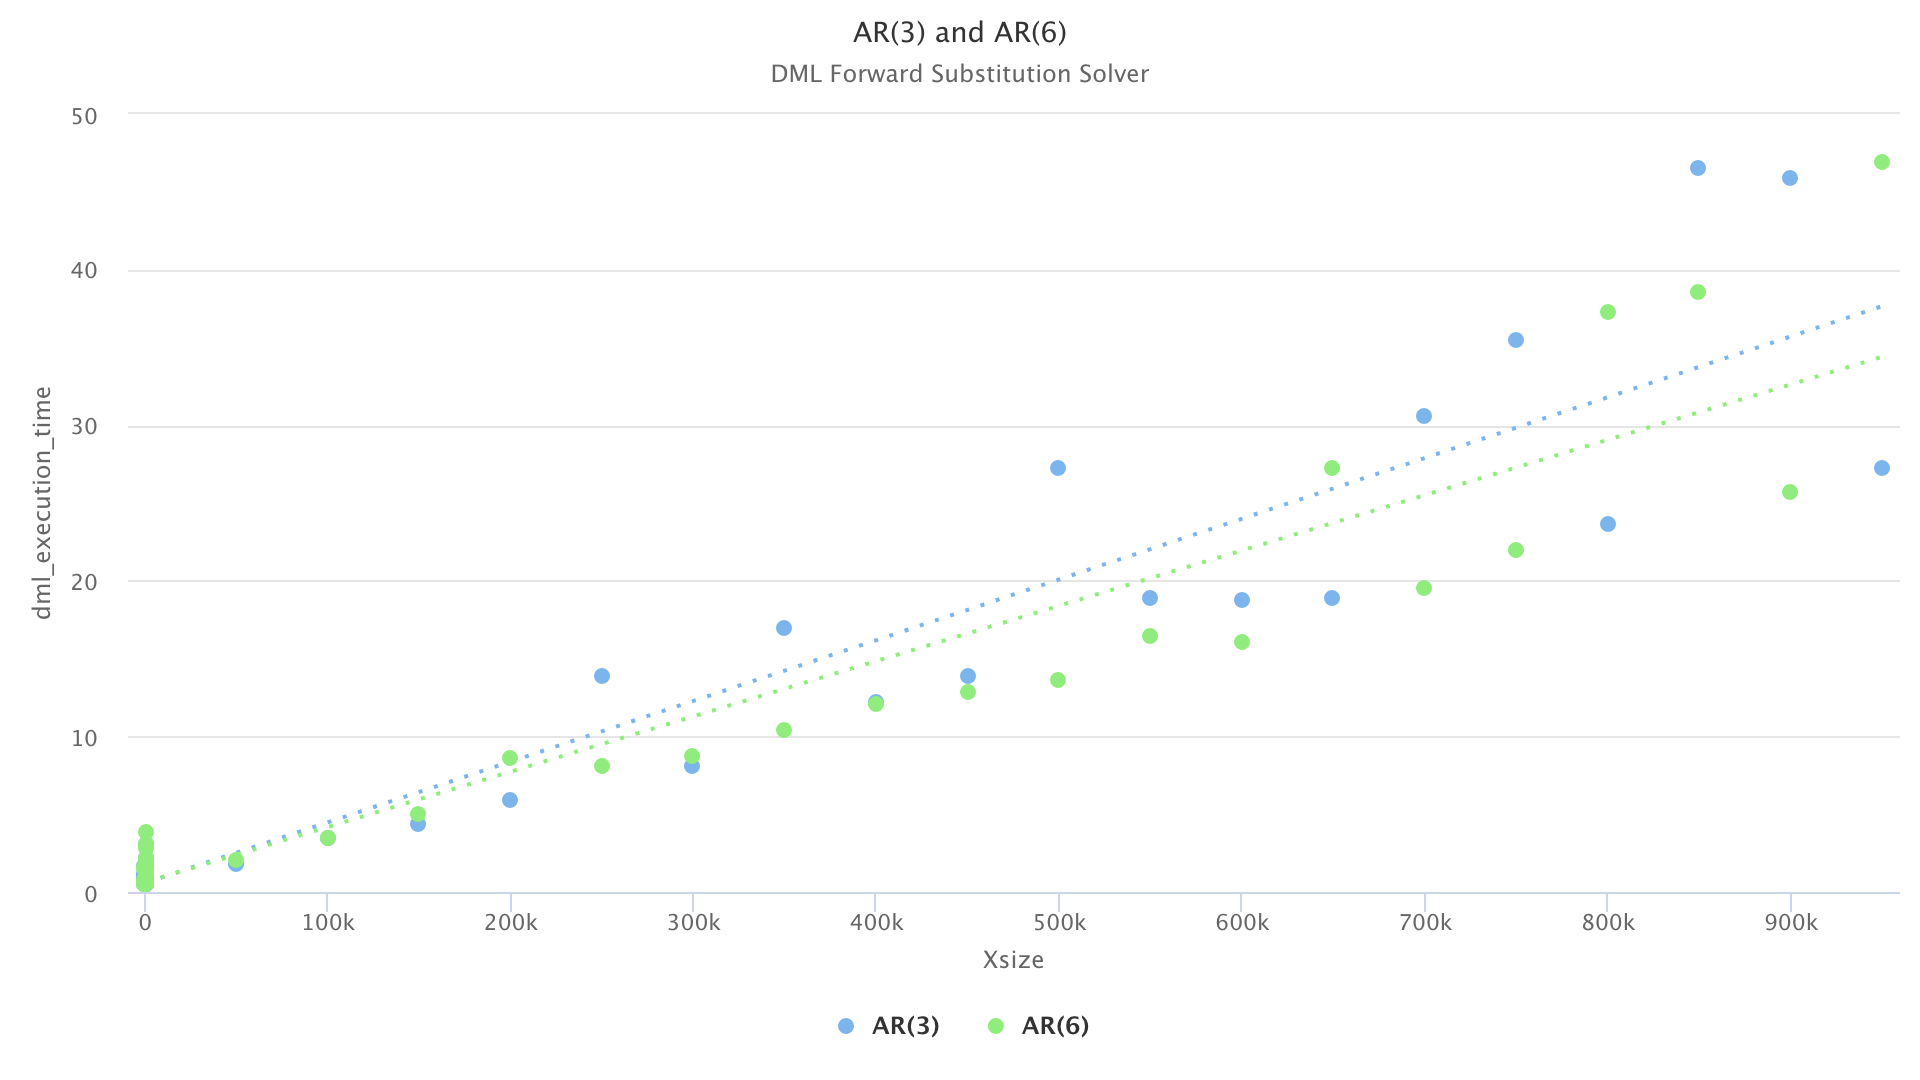
\includegraphics[width=\defaultsizeGraph]{images/ar-comparison-forwardsub.png}}
	\caption{Comparison of \textbf{Execution time} of \textbf{AR(3) and AR(6) for Forward Substitution DML} for time series with sizes \textbf{from $1,000$ up to $950,000$} }
    \label{apx-fig:ar-comparison-forwardsun}
\end{figure}

\begin{figure}[ht]
	\centering
	\scalebox{1}{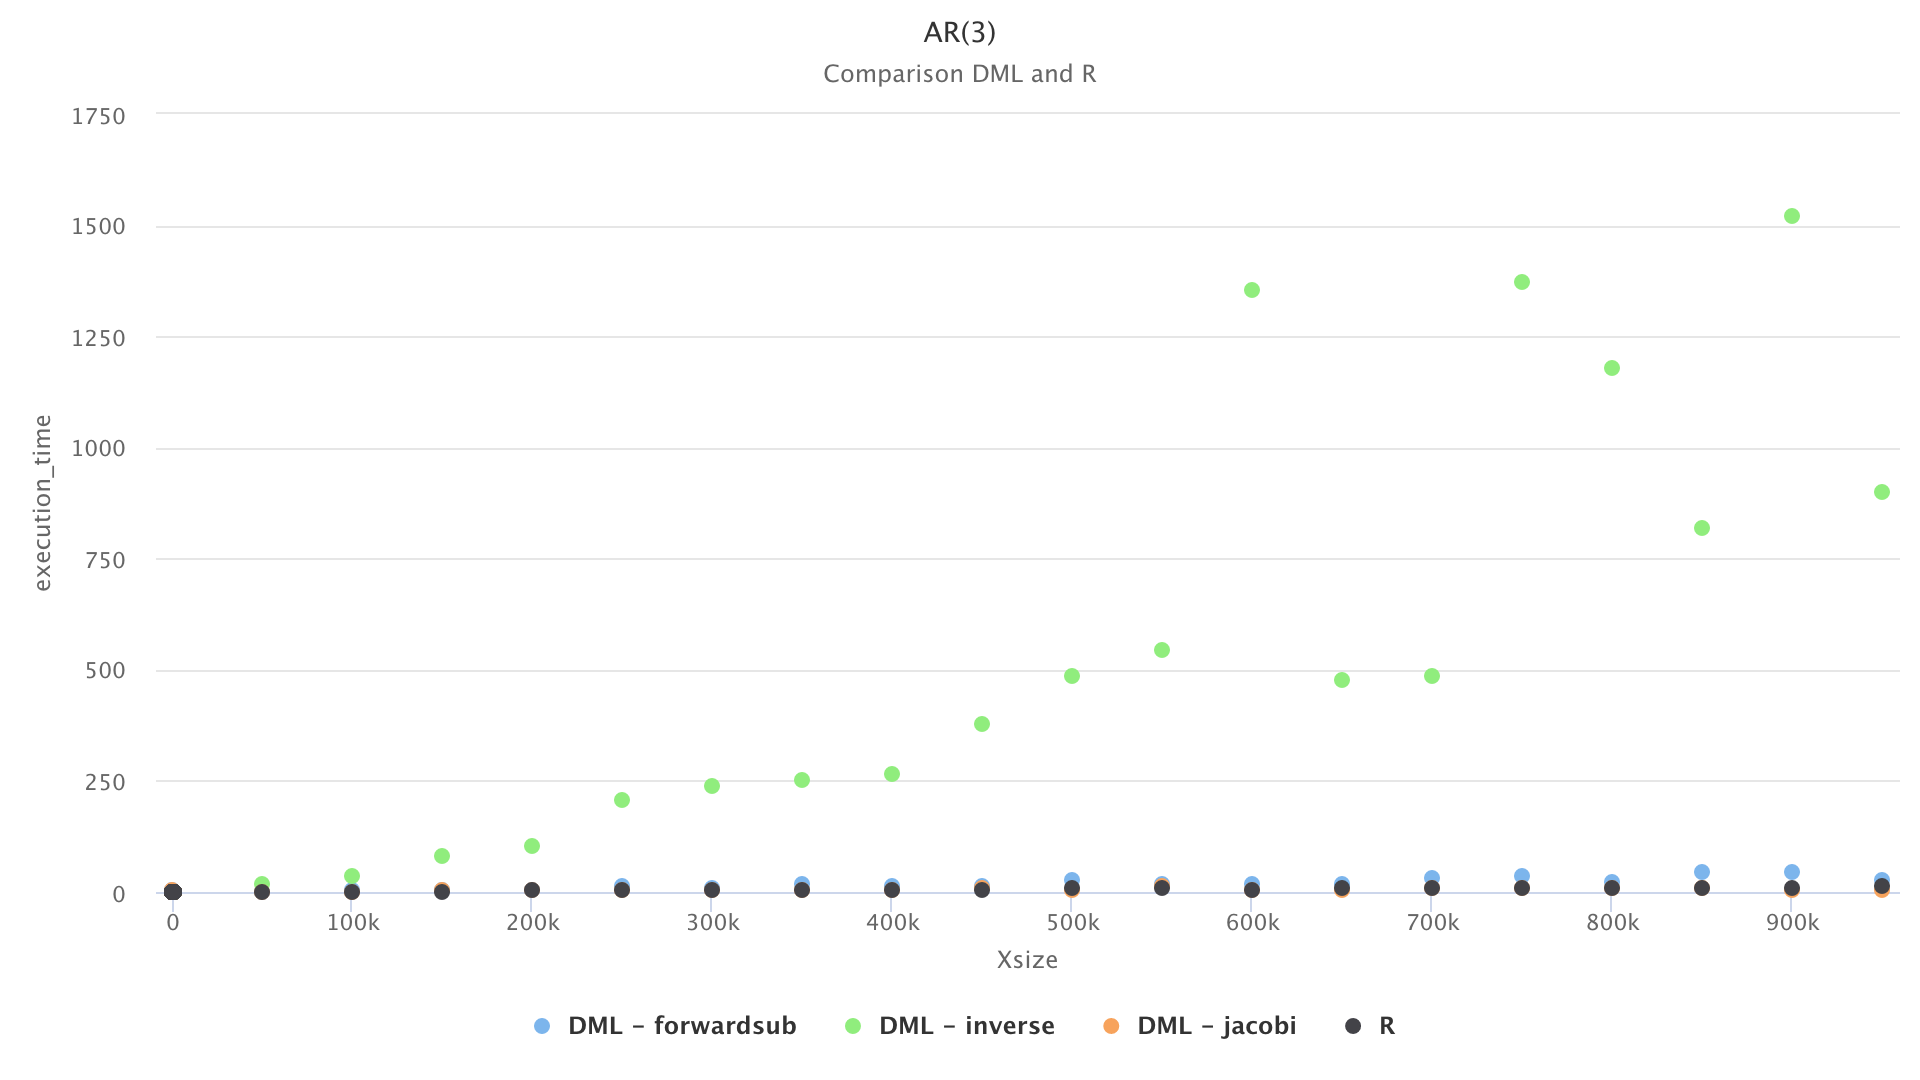
\includegraphics[width=\defaultsizeGraph]{images/ar3-exectime-scatter-all_big.png}}
	\caption{\textbf{Execution time} of AR(3) for DML and R for time series with sizes \textbf{up to $950,000$} }
    \label{apx-fig:ar3-exectime-scatter-all_big}
\end{figure}

\begin{figure}[ht]
	\centering
	\scalebox{1}{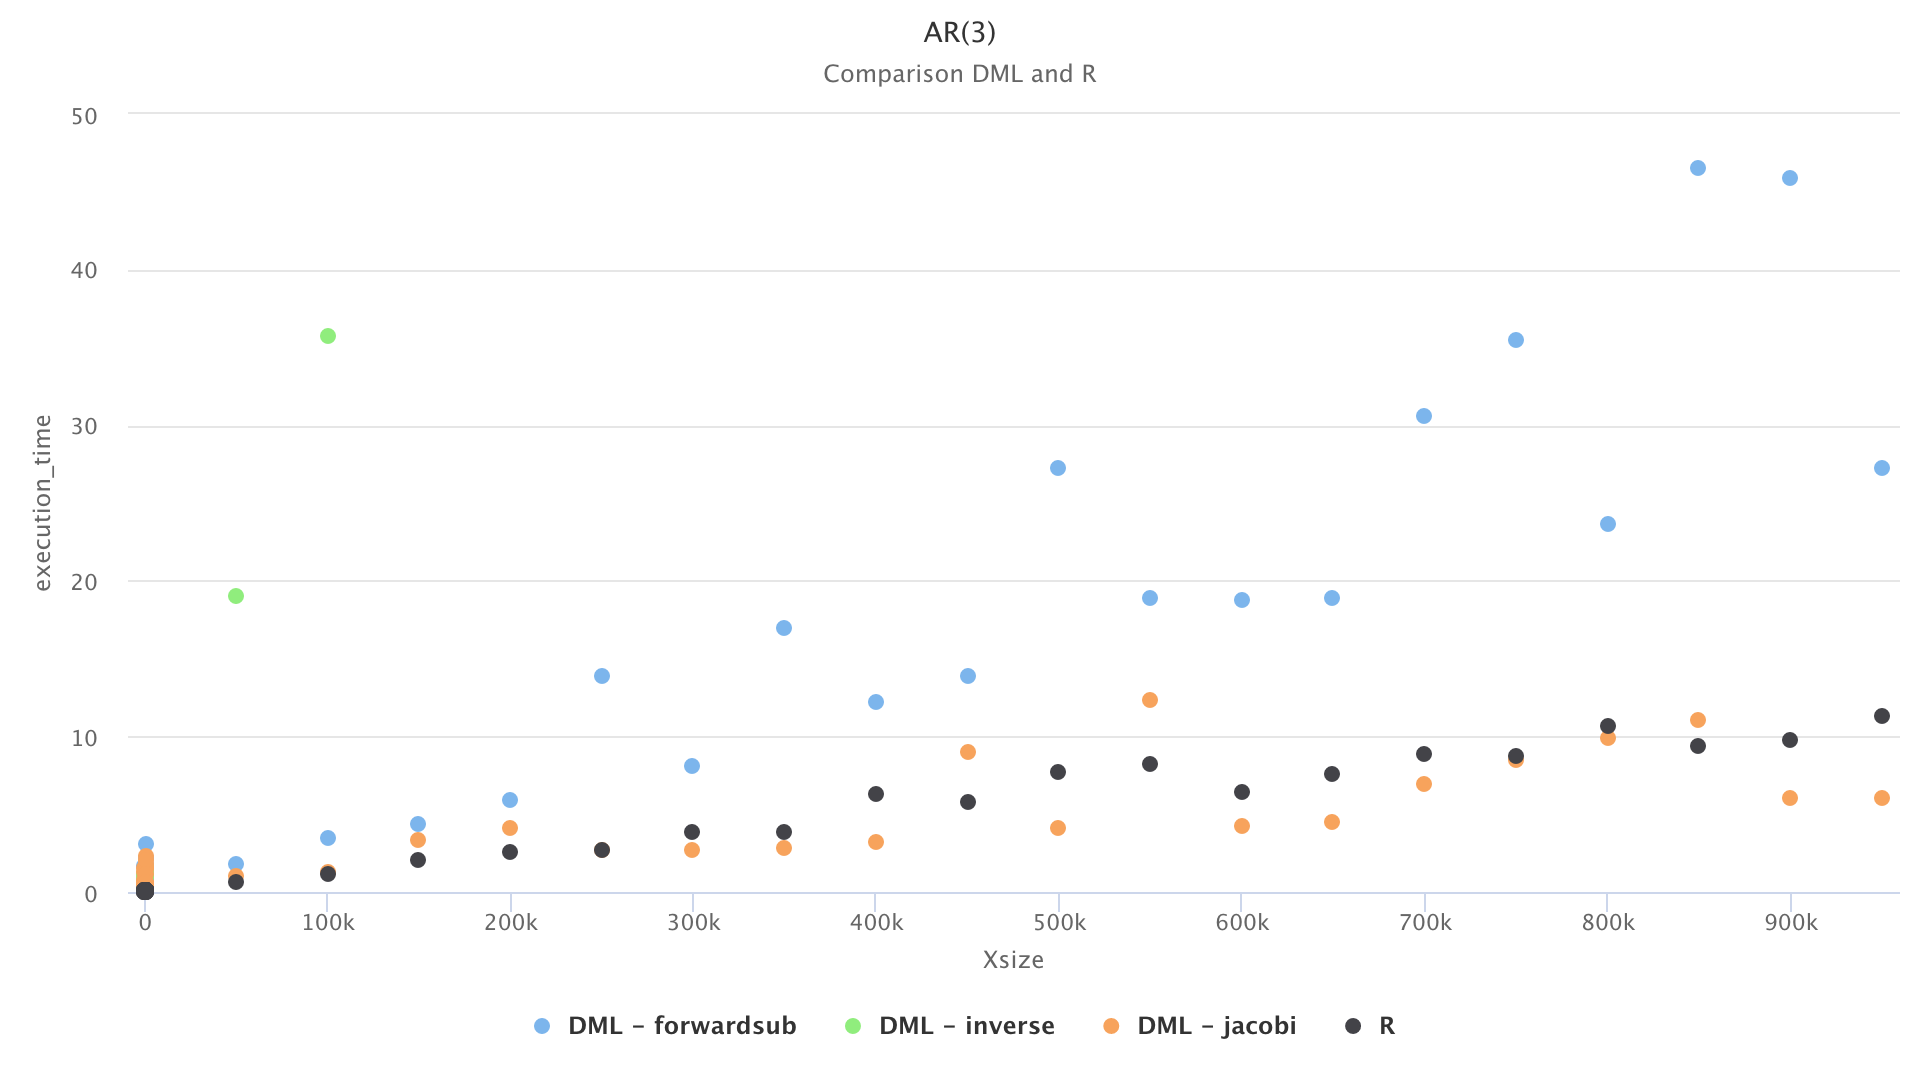
\includegraphics[width=\defaultsizeGraph]{images/ar3-exectime-scatter-all.png}}
	\caption{\textbf{Execution time} of AR(3) for DML and R for time series with sizes \textbf{up to $950,000$} but on a reduced time scale limited to}
    \label{apx-fig:ar3-exectime-scatter-all}
\end{figure}

\begin{figure}[ht]
	\centering
	\scalebox{1}{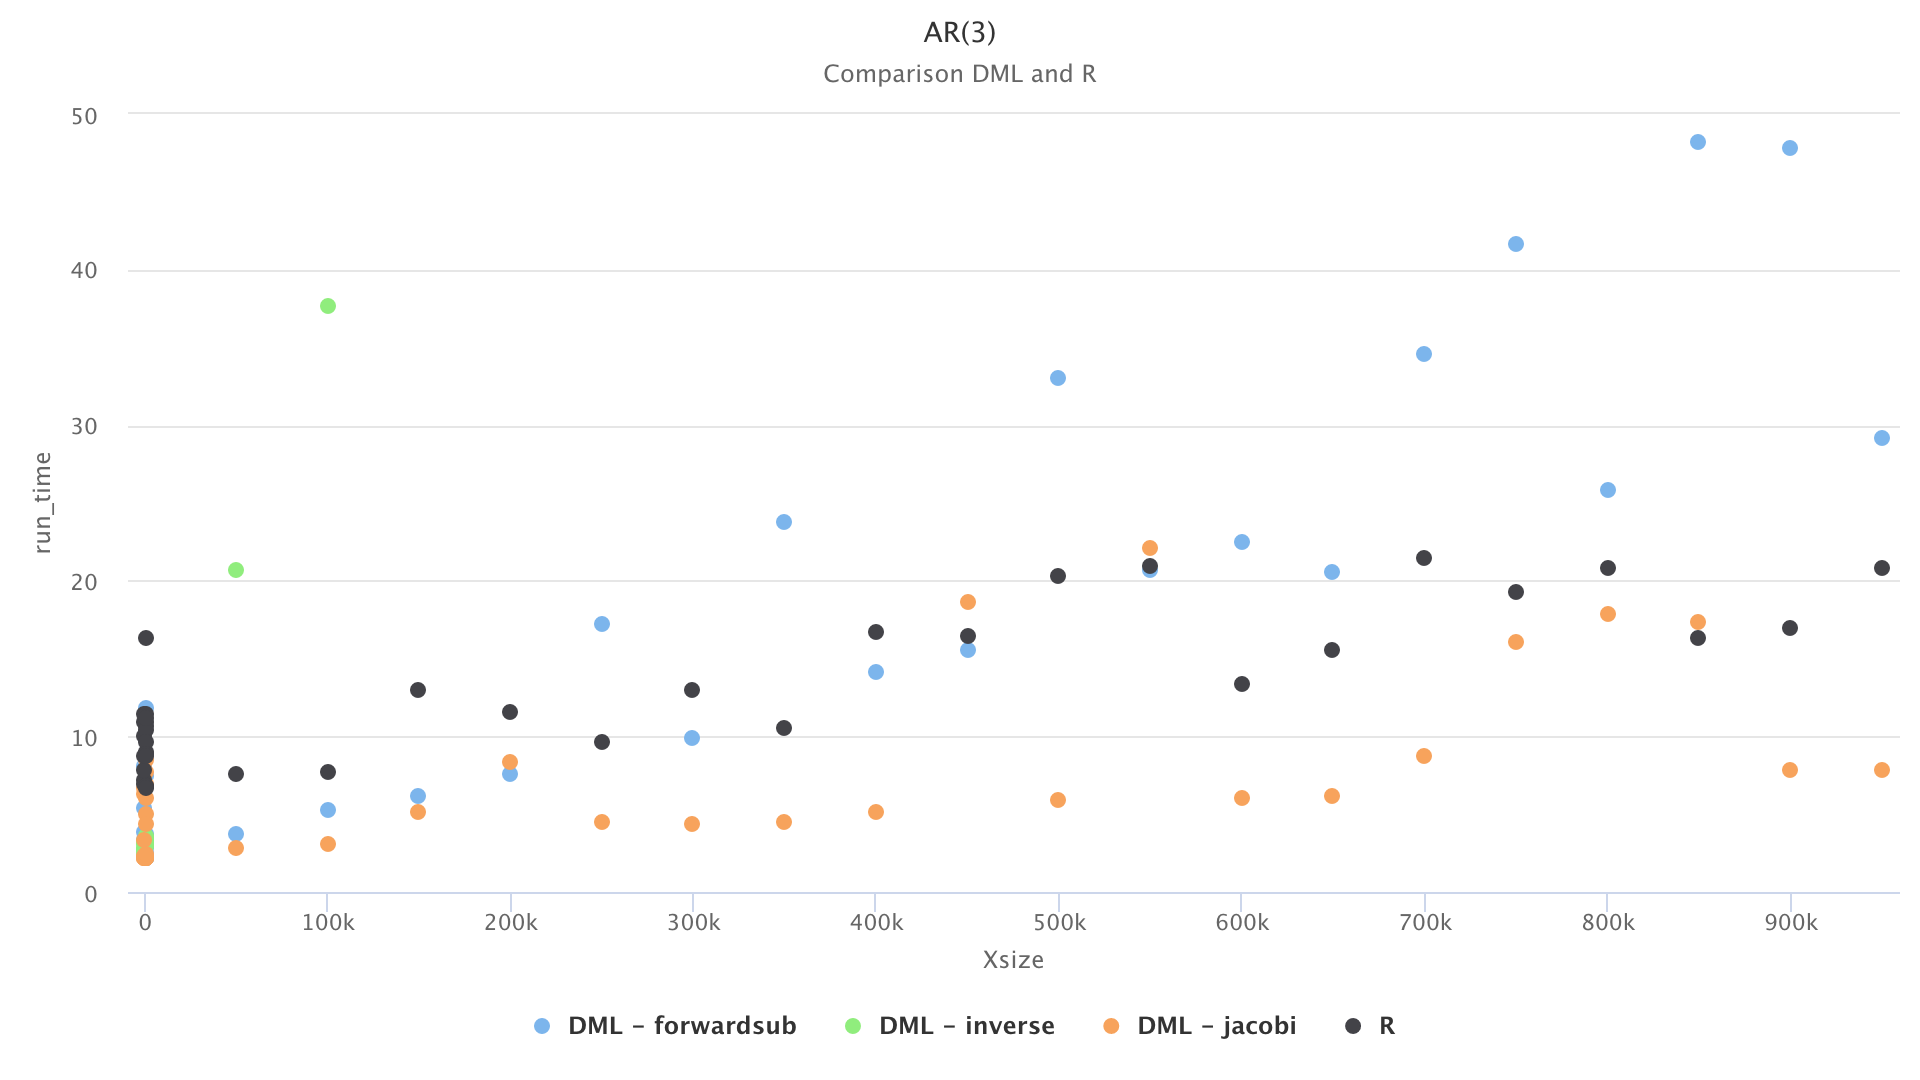
\includegraphics[width=\defaultsizeGraph]{images/ar3-runtime-scatter-all.png}}
	\caption{\textbf{Run time of} AR(3) for DML and R for time series with sizes \textbf{up to $950,000$} }
    \label{apx-fig:ar3-runtime-scatter-all}
\end{figure}

\begin{figure}[ht]
	\centering
	\scalebox{1}{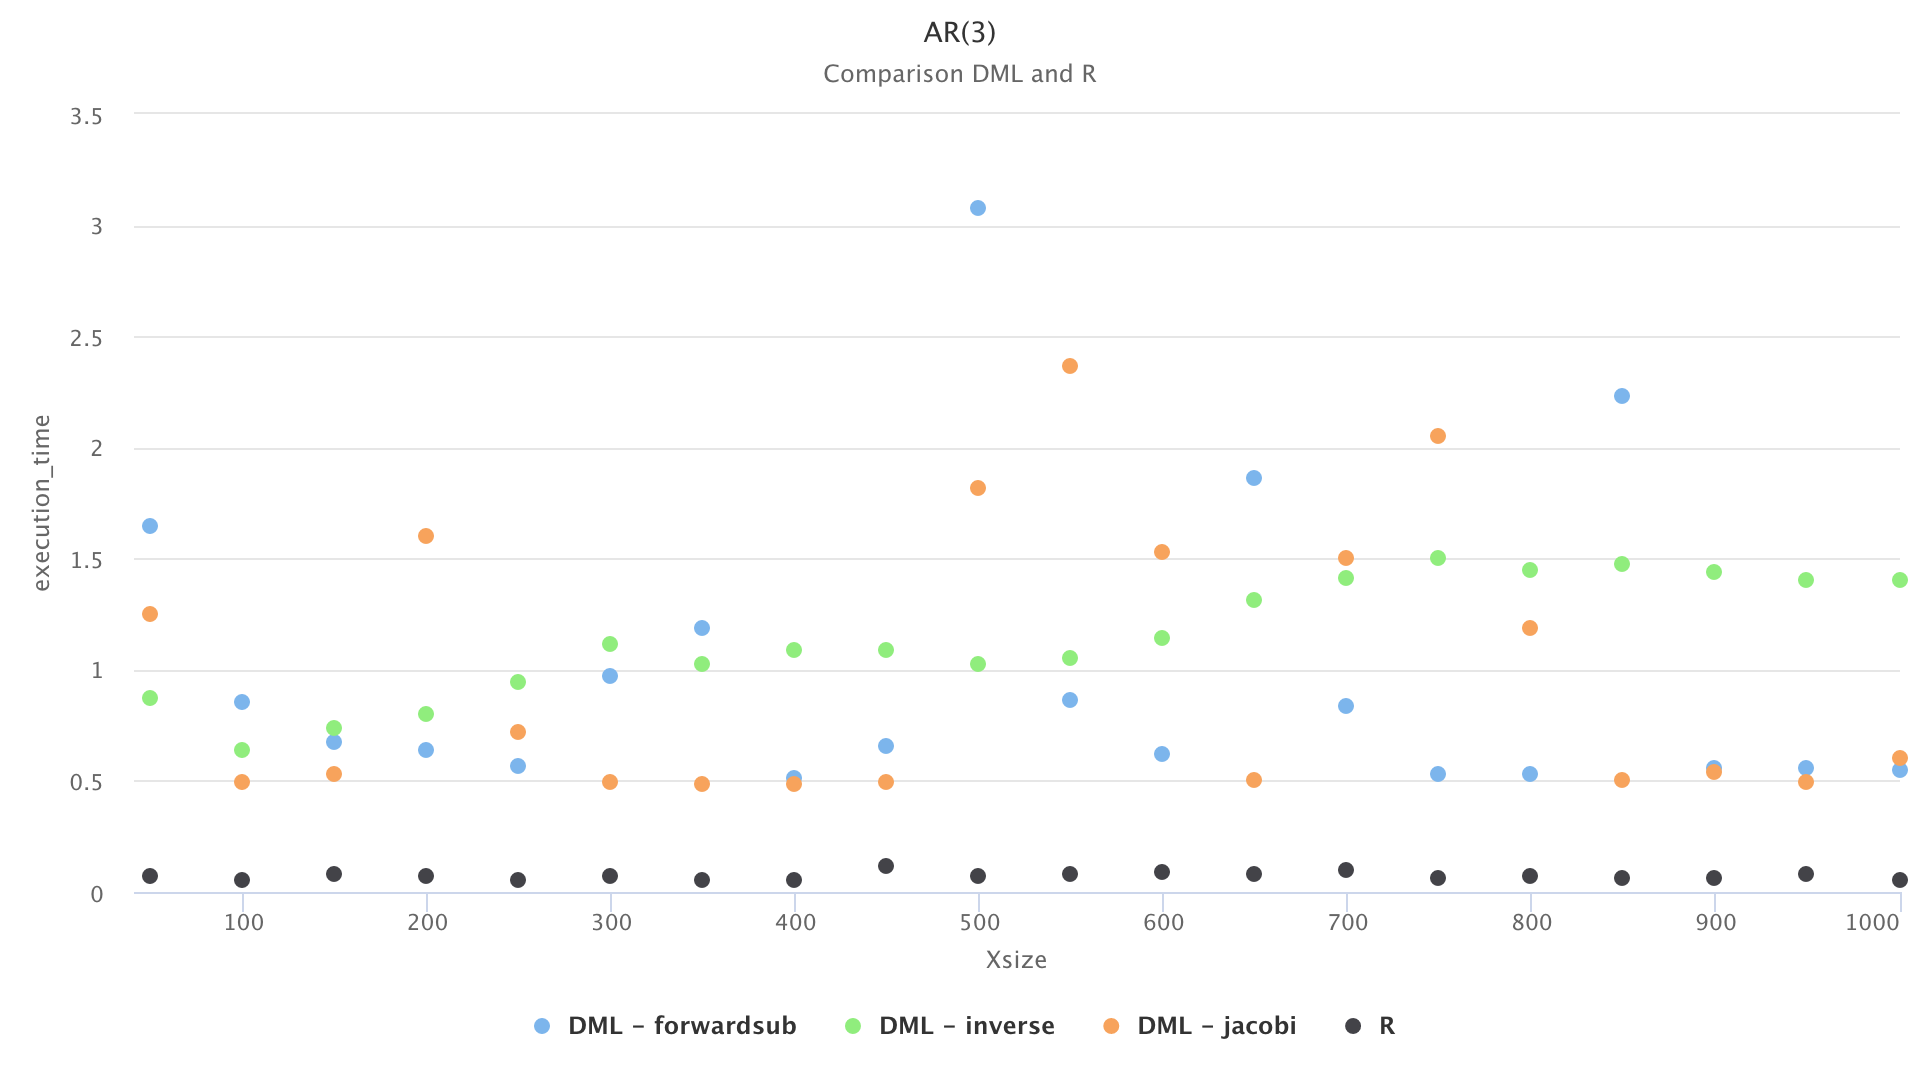
\includegraphics[width=\defaultsizeGraph]{images/ar3-exectime-scatter-all_small.png}}
	\caption{\textbf{Execution time} of AR(3) for DML and R for time series with sizes \textbf{from $50$ to $1,000$} }
    \label{apx-fig:ar3-exectime-scatter-all_small}
\end{figure}

\begin{figure}[ht]
	\centering
	\scalebox{1}{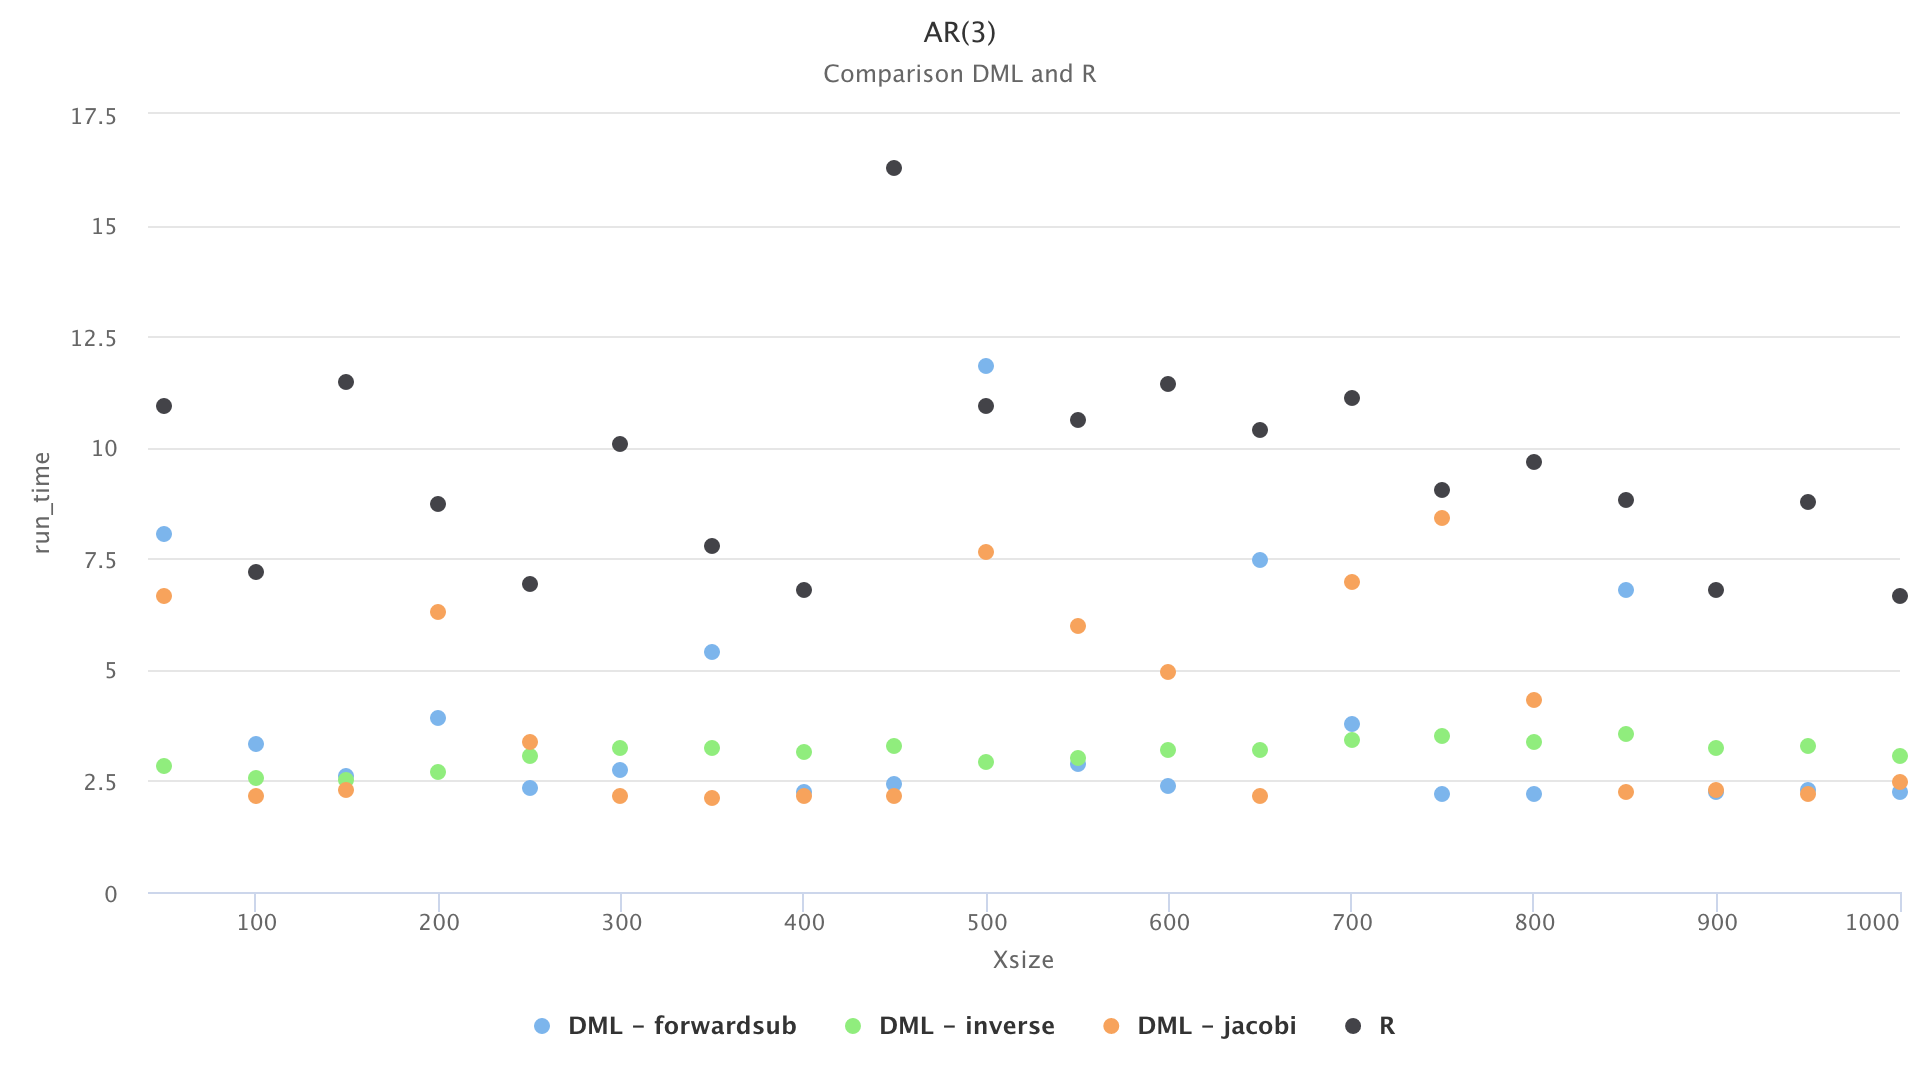
\includegraphics[width=\defaultsizeGraph]{images/ar3-runtime-scatter-all_small.png}}
	\caption{\textbf{Run time} of AR(3) for DML and R for time series with sizes \textbf{from $50$ to $1,000$} }
    \label{apx-fig:ar3-runtime-scatter-all_small}
\end{figure}


\begin{figure}[ht]
	\centering
	\scalebox{1}{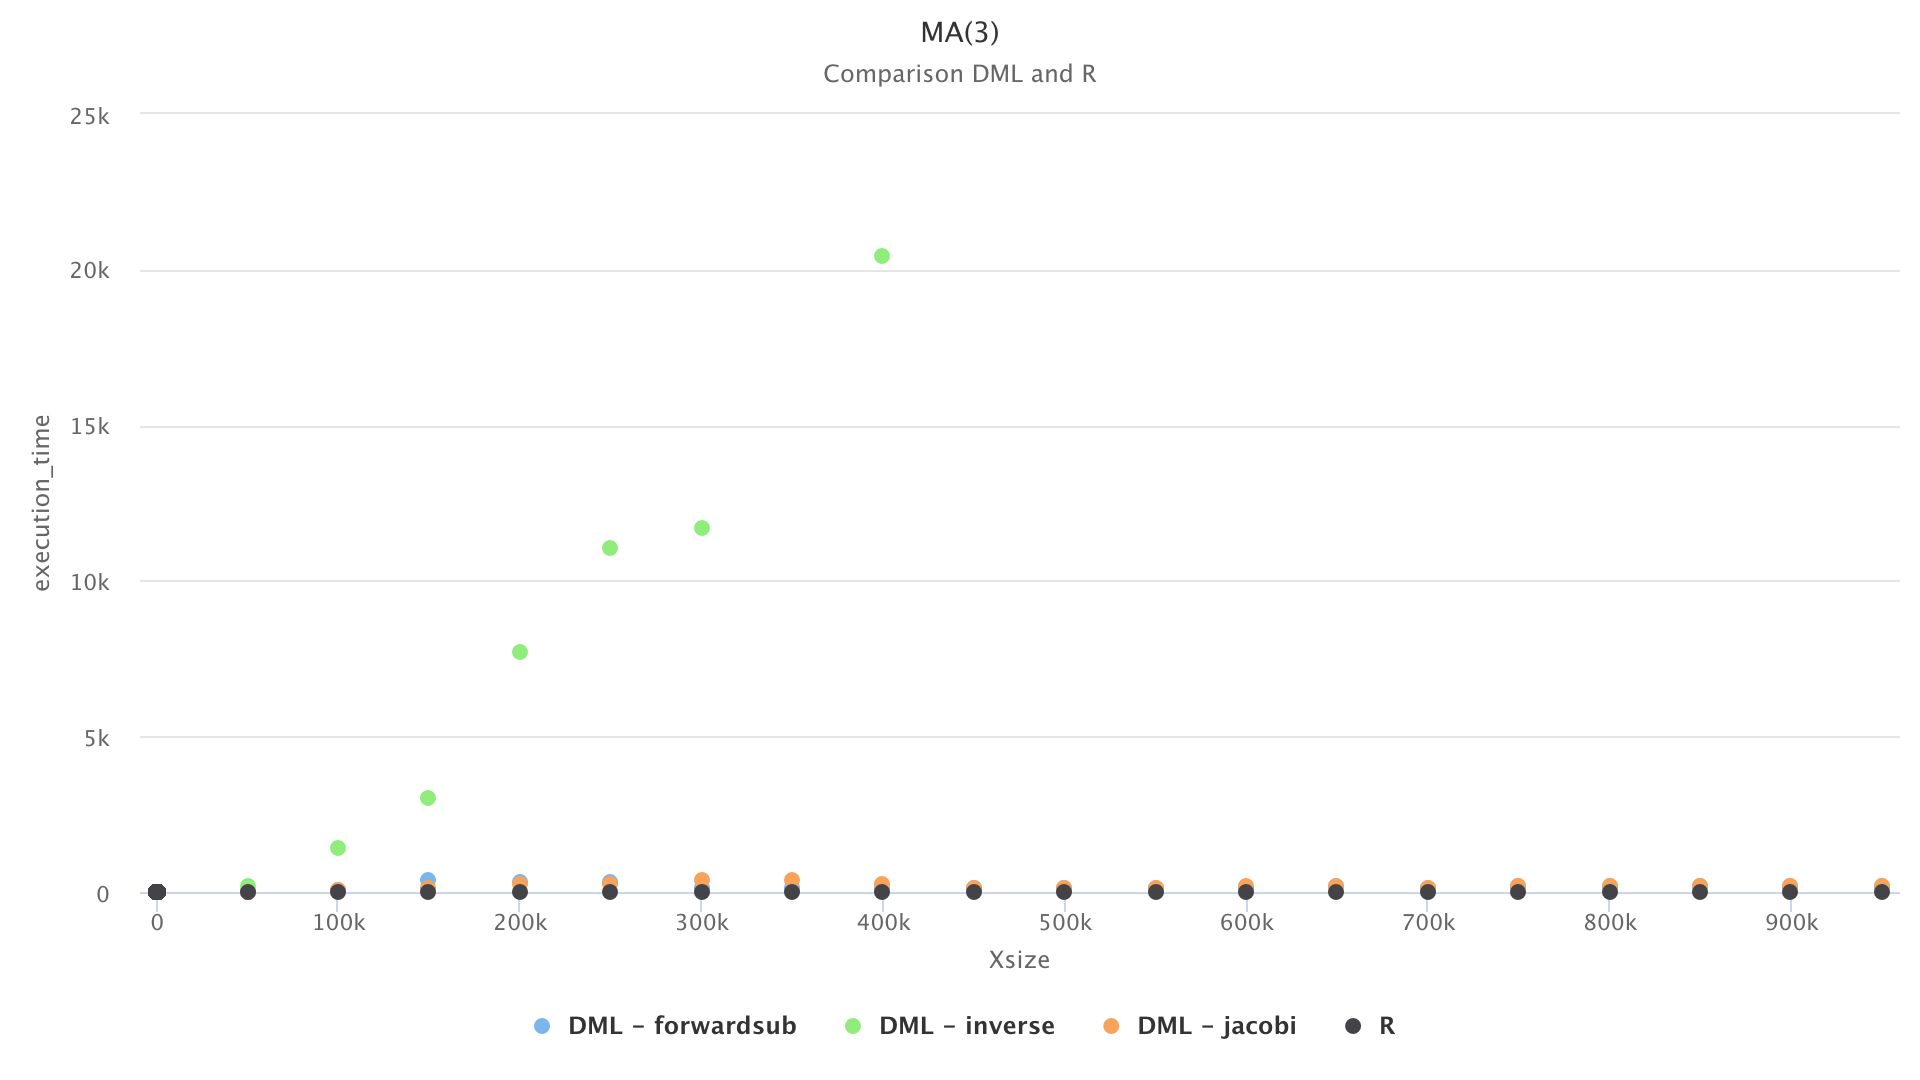
\includegraphics[width=\defaultsizeGraph]{images/ma3-exectime-scatter-all.png}}
	\caption{\textbf{Execution time} of MA(3) for DML and R for time series with sizes \textbf{up to $950,000$} }
    \label{apx-fig:ma3-exectime-scatter-all}
\end{figure}

\begin{figure}[ht]
	\centering
	\scalebox{1}{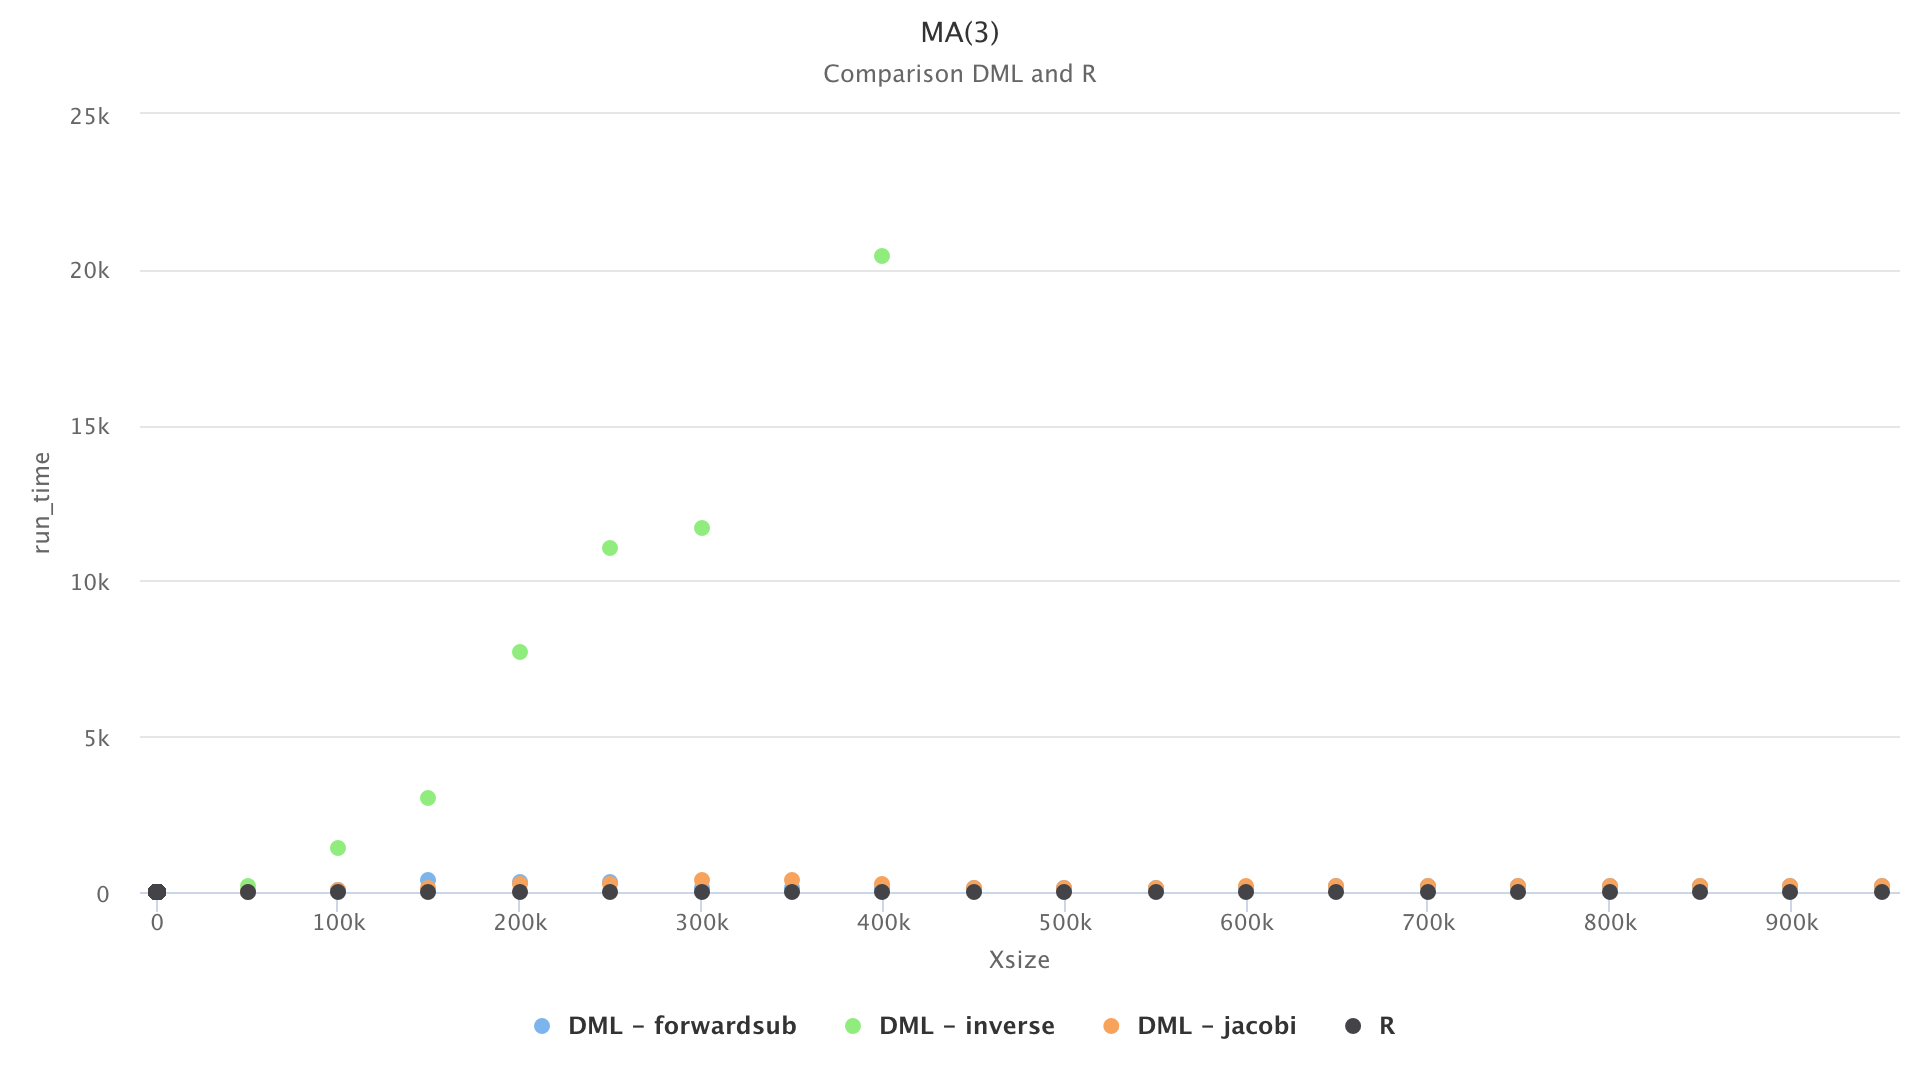
\includegraphics[width=\defaultsizeGraph]{images/ma3-runtime-scatter-all.png}}
	\caption{\textbf{Run time of} MA(3) for DML and R for time series with sizes \textbf{up to $950,000$} }
    \label{apx-fig:ma3-runtime-scatter-all}
\end{figure}

\begin{figure}[ht]
	\centering
	\scalebox{1}{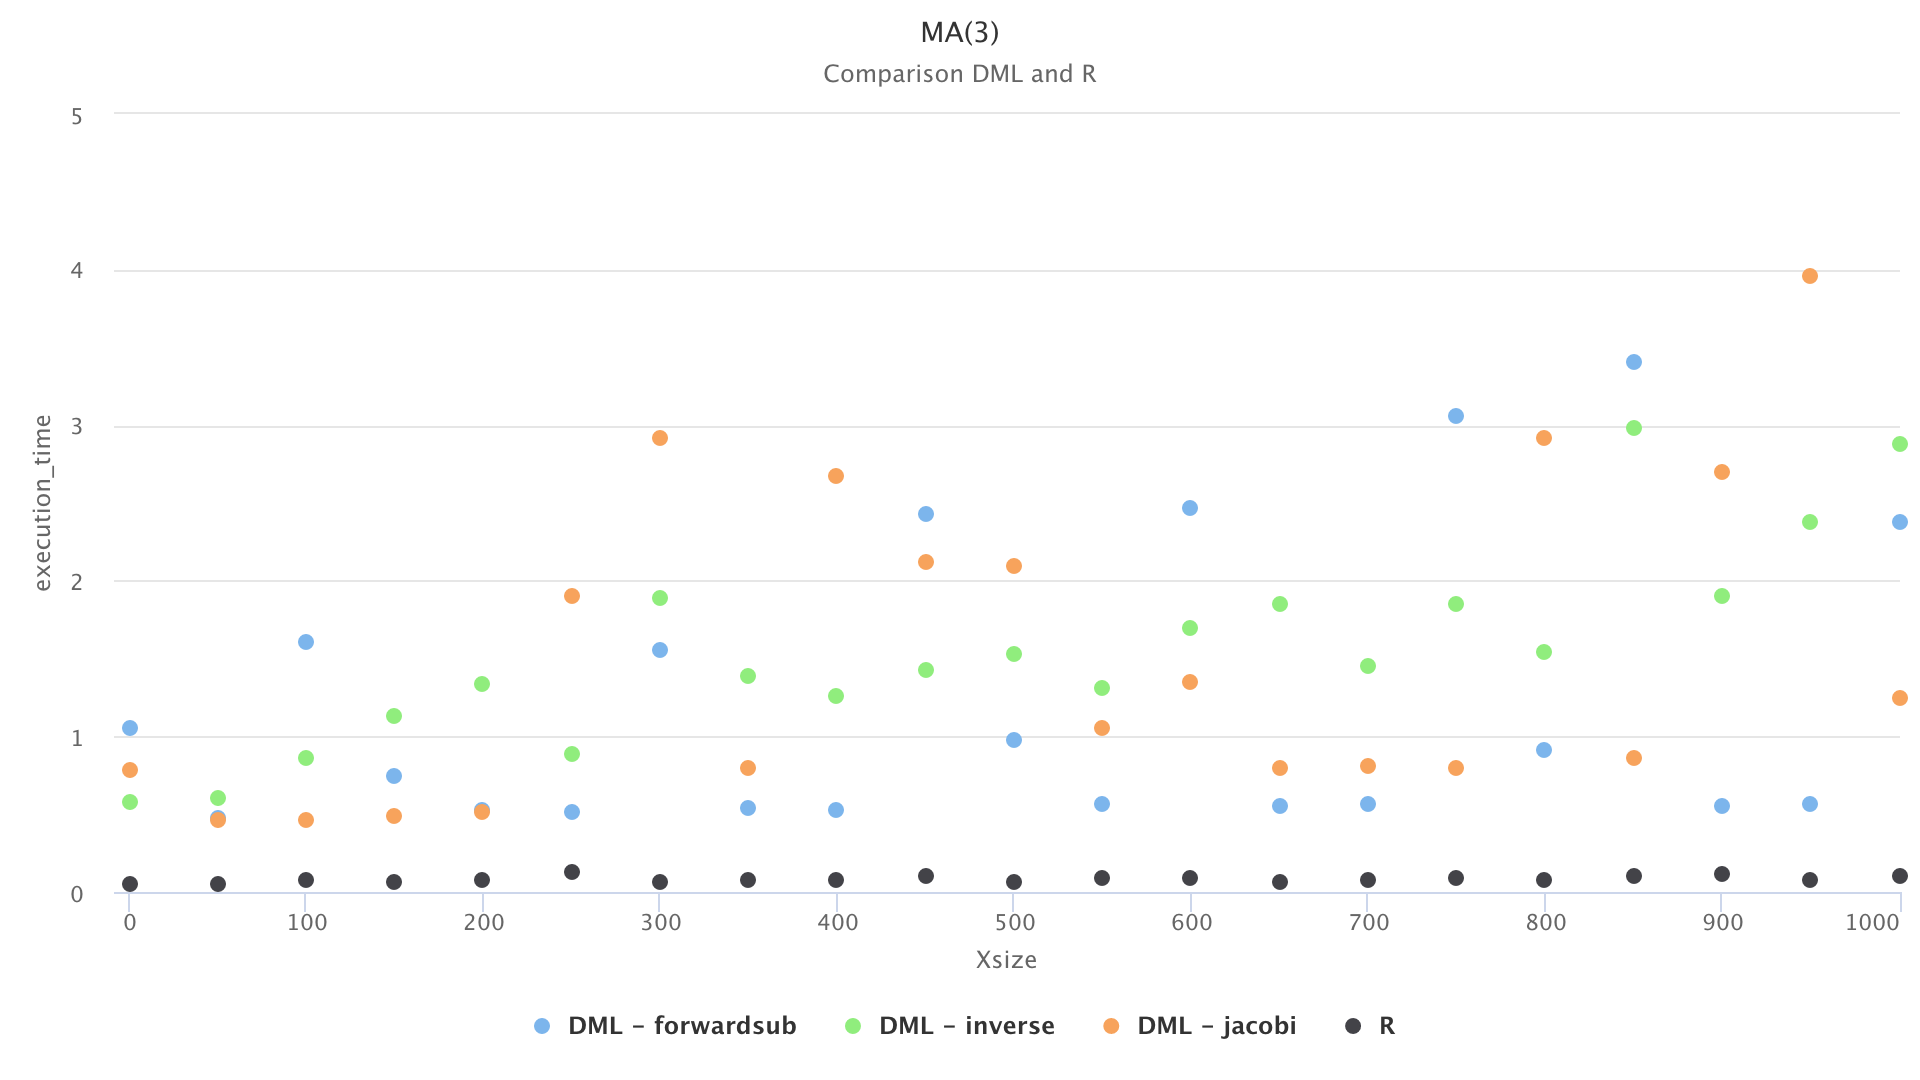
\includegraphics[width=\defaultsizeGraph]{images/ma3-exectime-scatter-all_small.png}}
	\caption{\textbf{Execution time} of MA(3) for DML and R for time series with sizes \textbf{from $50$ to $1,000$} }
    \label{apx-fig:ma3-exectime-scatter-all_small}
\end{figure}

\begin{figure}[ht]
	\centering
	\scalebox{1}{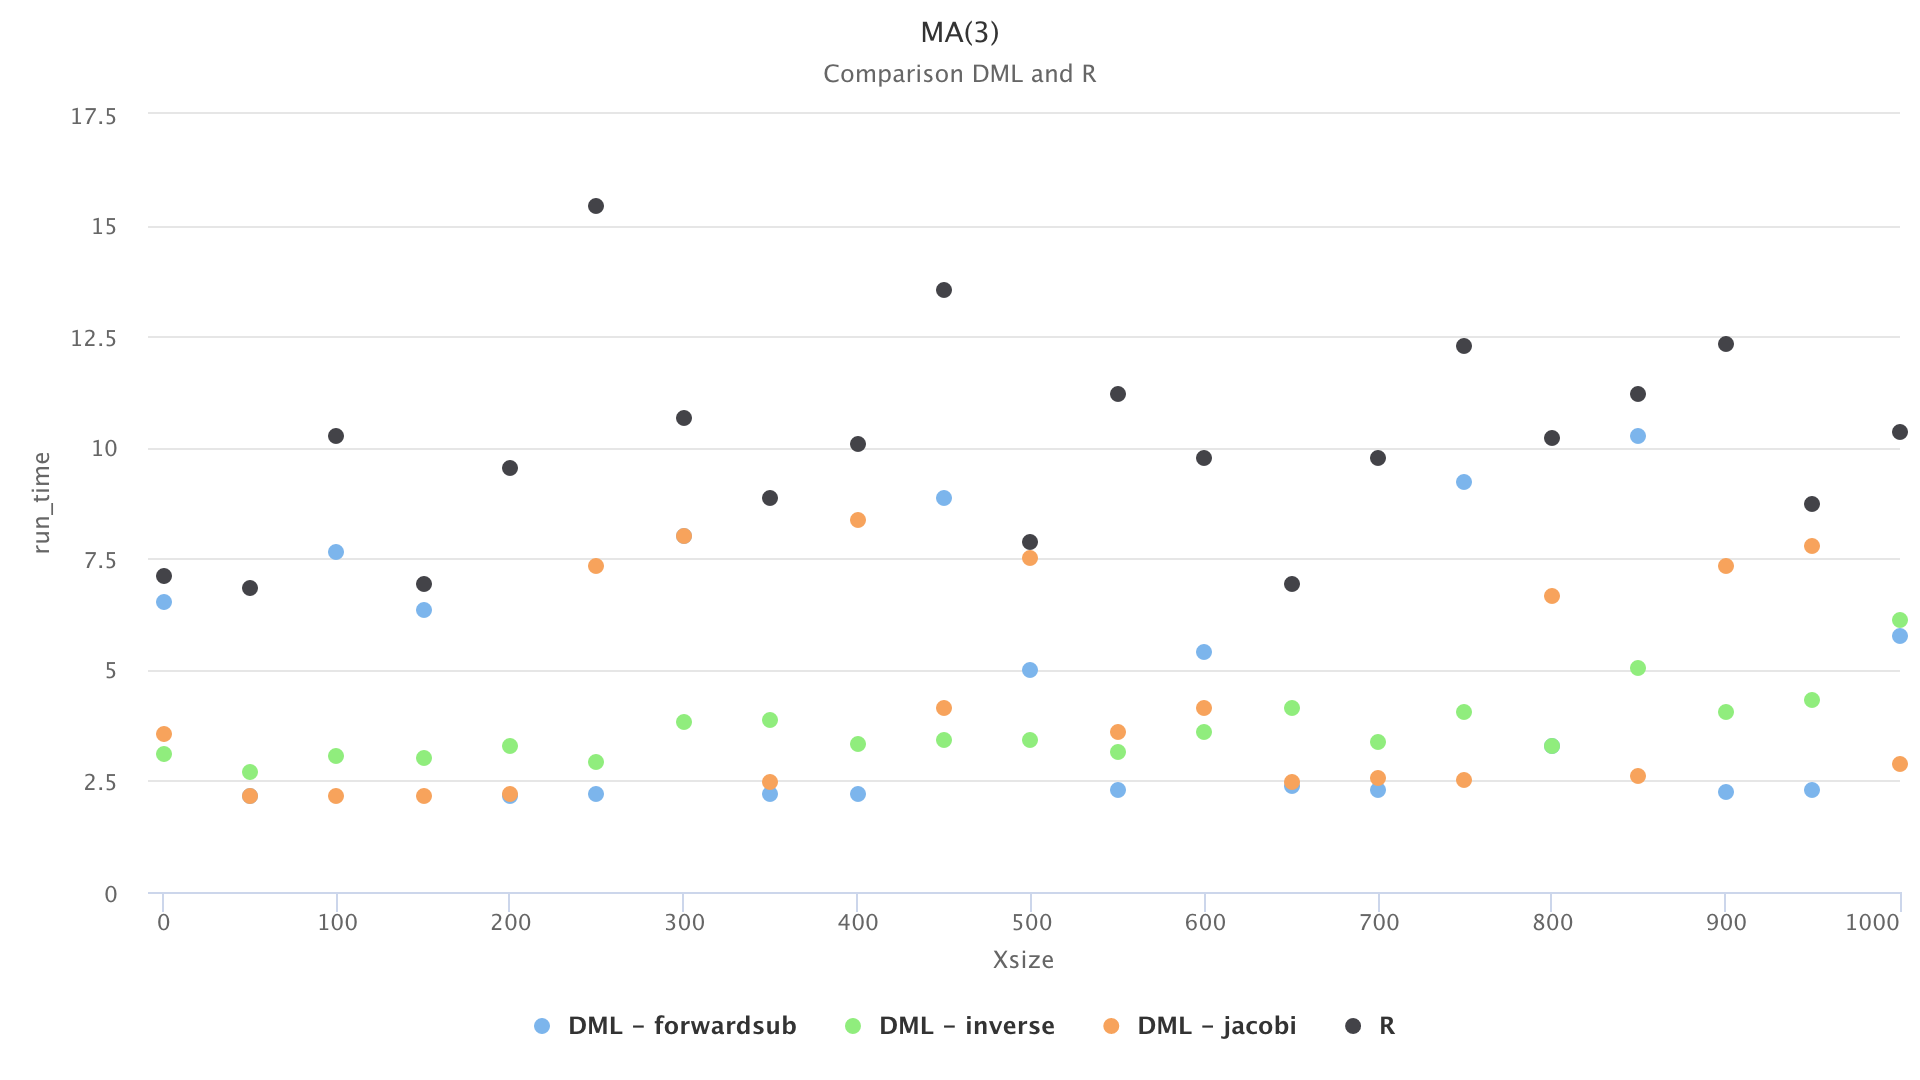
\includegraphics[width=\defaultsizeGraph]{images/ma3-runtime-scatter-all_small.png}}
	\caption{\textbf{Run time} of MA(3) for DML and R for time series with sizes \textbf{from $50$ to $1,000$}}
    \label{apx-fig:ma3-runtime-scatter-all_small}
\end{figure}


\begin{figure}[ht]
	\centering
	\scalebox{1}{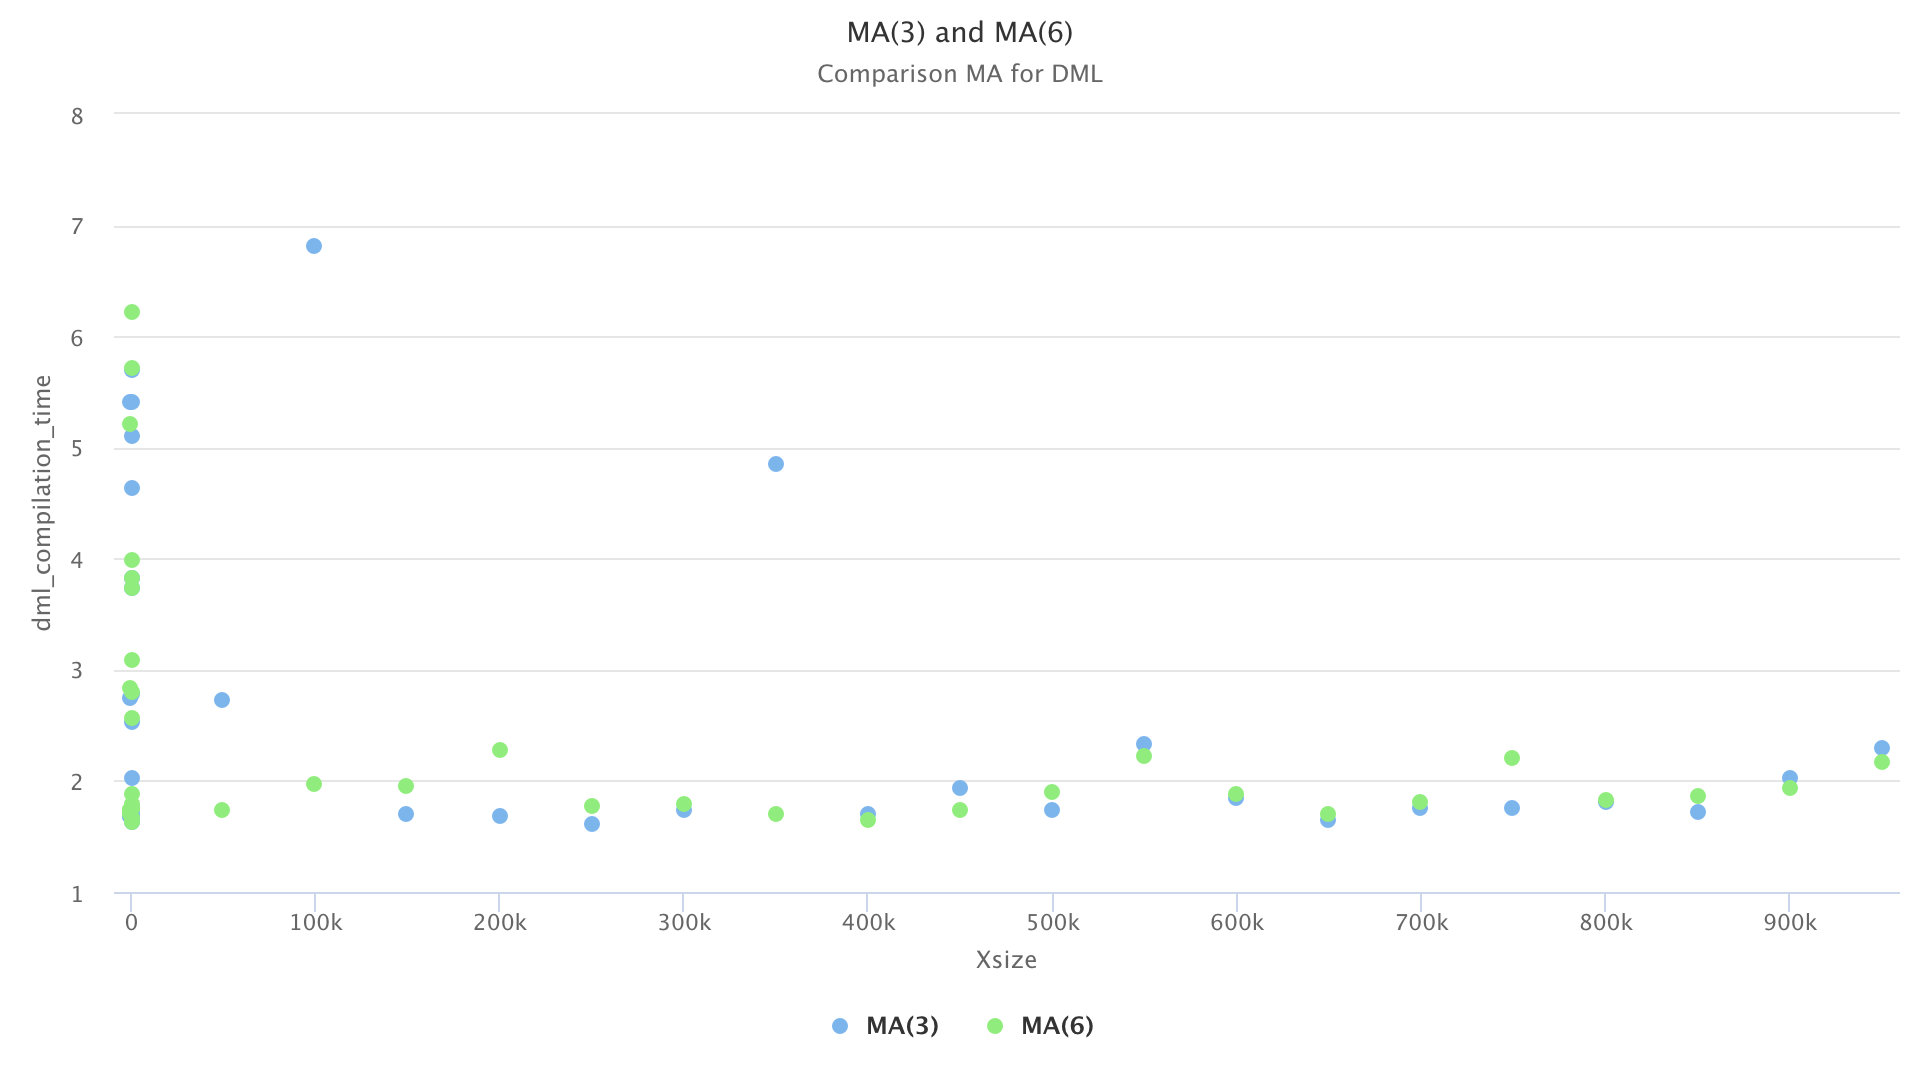
\includegraphics[width=\defaultsizeGraph]{images/ma-comparison.png}}
	\caption{Comparison of DML \textbf{execution time} of MA(3) and MA(6) - \textit{average of all solvers}}
    \label{apx-fig:ma-comparison}
\end{figure}


\begin{figure}[ht]
	\centering
	\scalebox{1}{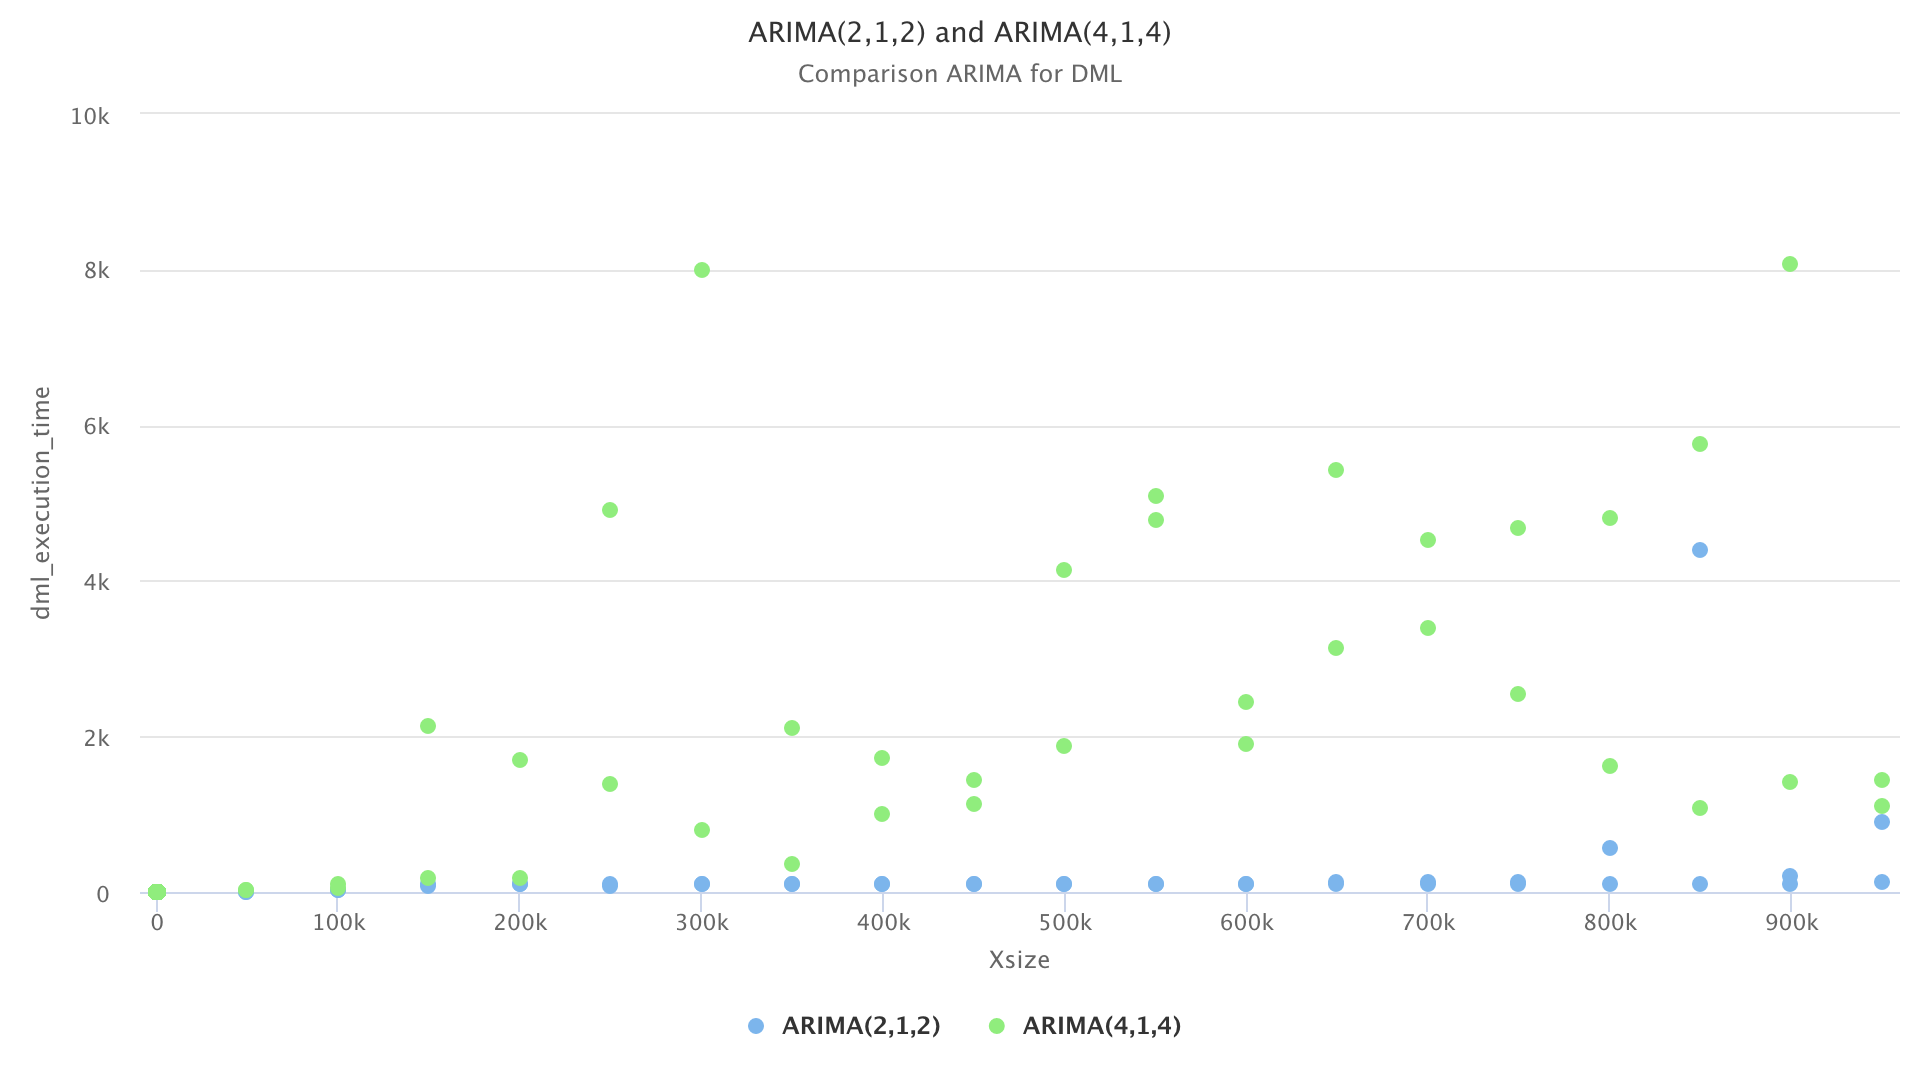
\includegraphics[width=\defaultsizeGraph]{images/arima-comparison.png}}
	\caption{Comparison of DML \textbf{execution time} of ARIMA(2,1,2) and ARIMA(4,1,4) - \textit{average of all solvers}}
    \label{apx-fig:arima-comparison}
\end{figure}


\begin{figure}[ht]
	\centering
	\scalebox{1}{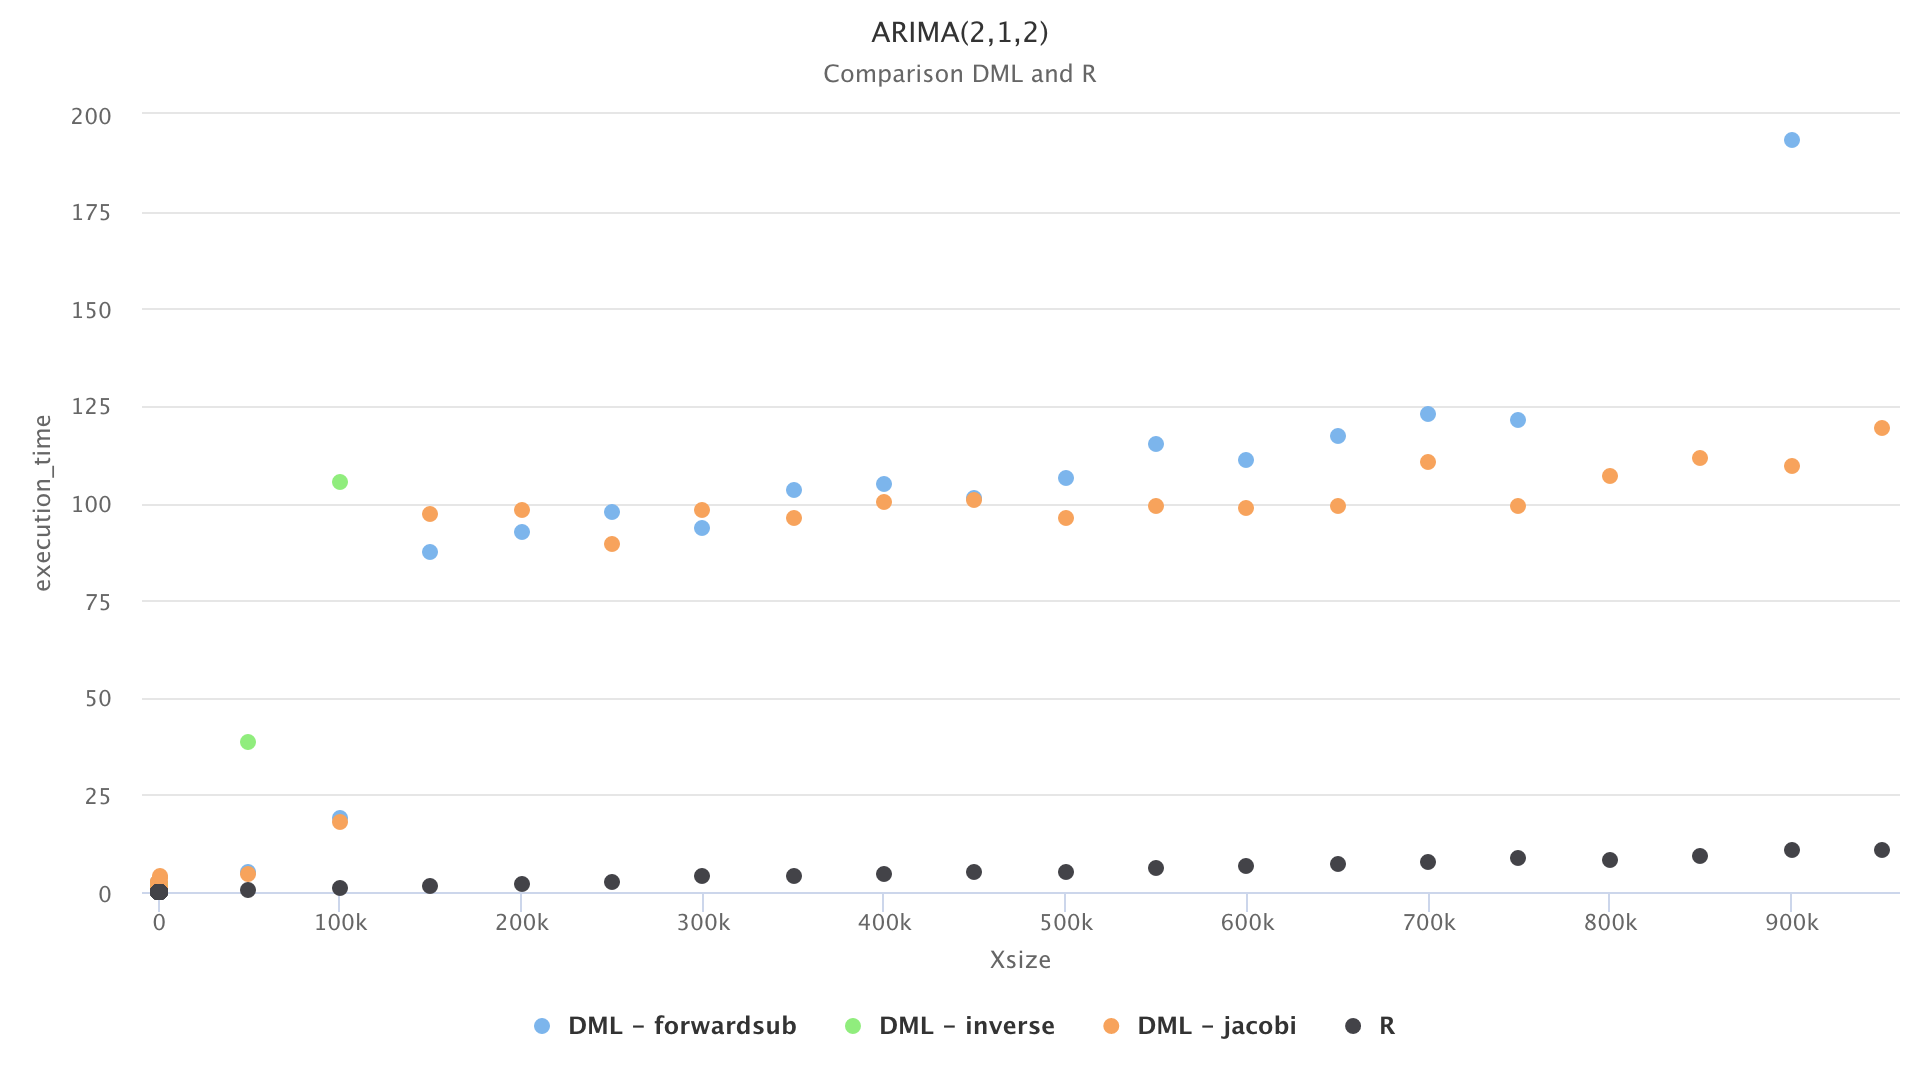
\includegraphics[width=\defaultsizeGraph]{images/arima212-exectime-scatter-all.png}}
	\caption{\textbf{Execution time} of ARIMA(2,1,2) for DML and R for time series with sizes \textbf{up to $950,000$} }
    \label{apx-fig:arima212-exectime-scatter-all}
\end{figure}

\begin{figure}[ht]
	\centering
	\scalebox{1}{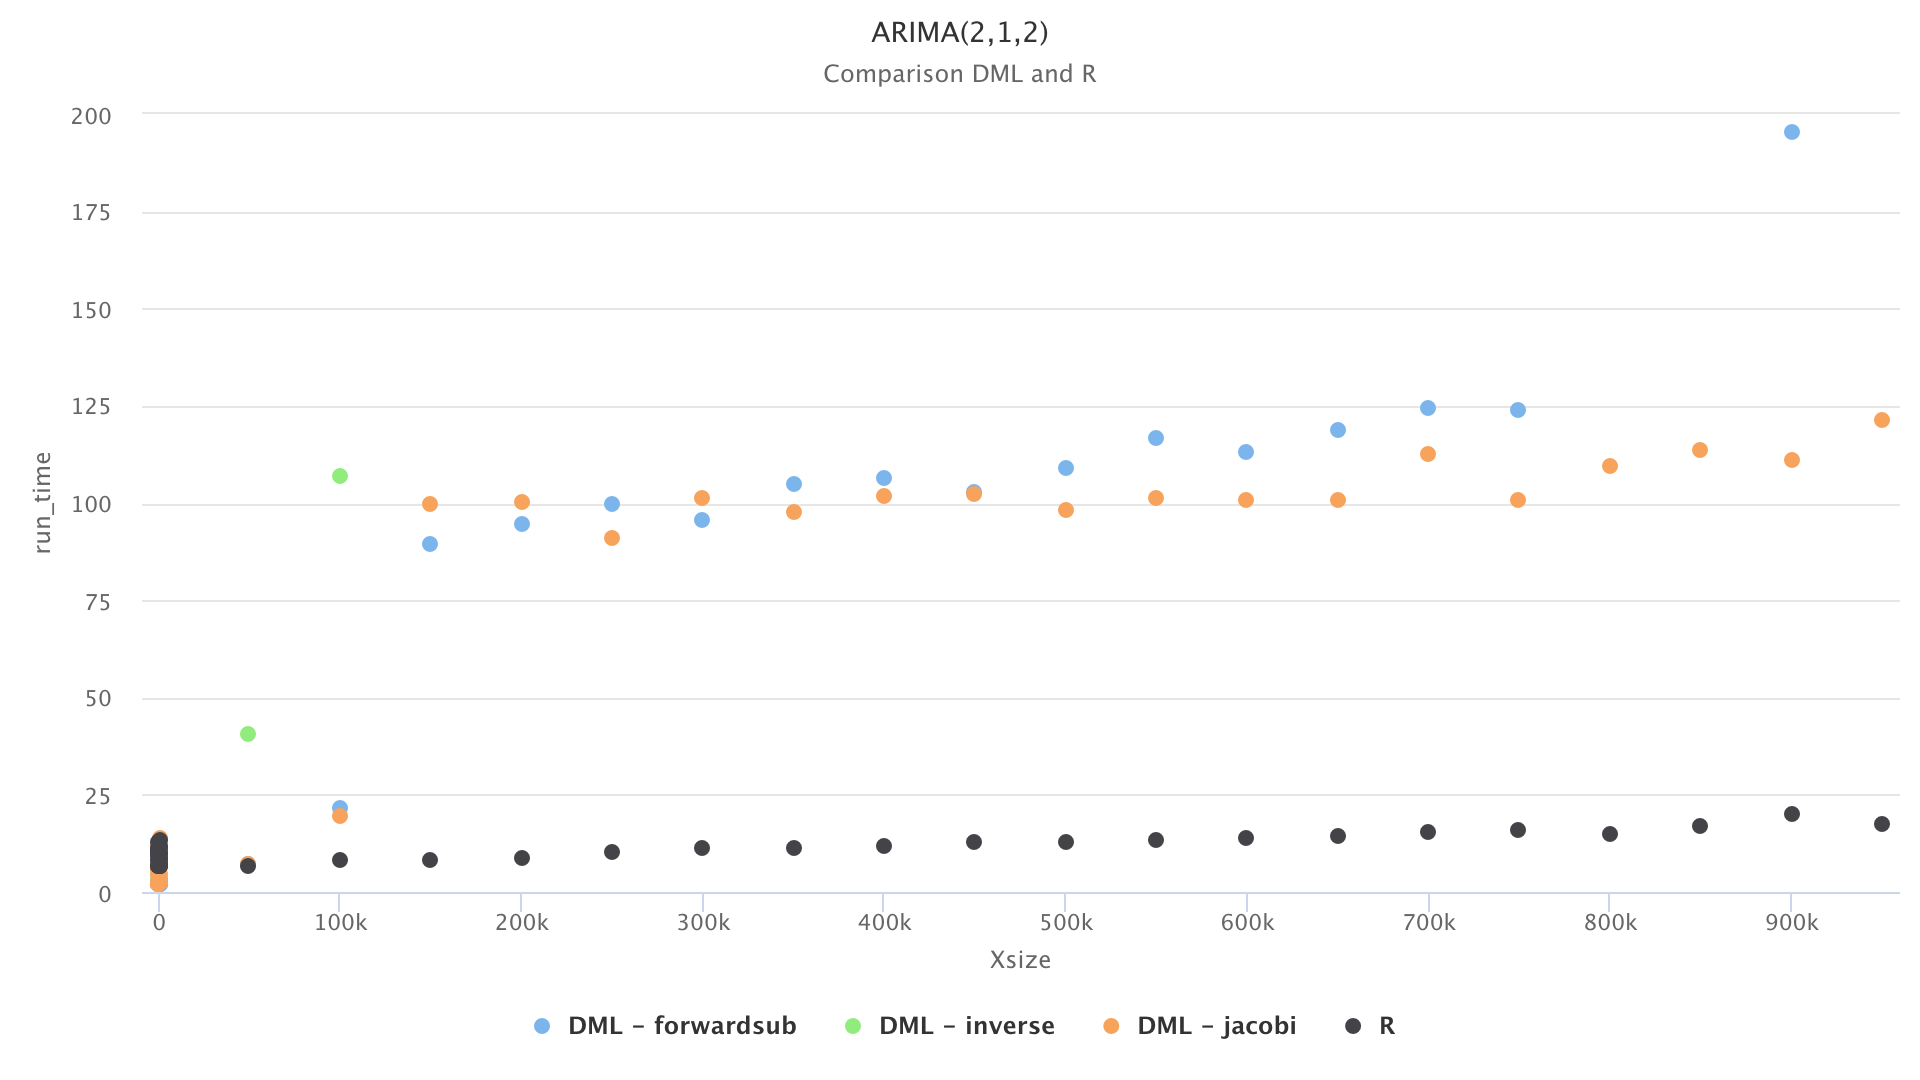
\includegraphics[width=\defaultsizeGraph]{images/arima212-runtime-scatter-all.png}}
	\caption{\textbf{Run time of} ARIMA(2,1,2) for DML and R for time series with sizes \textbf{up to $950,000$} }
    \label{apx-fig:arima212-runtime-scatter-all}
\end{figure}

\begin{figure}[ht]
	\centering
	\scalebox{1}{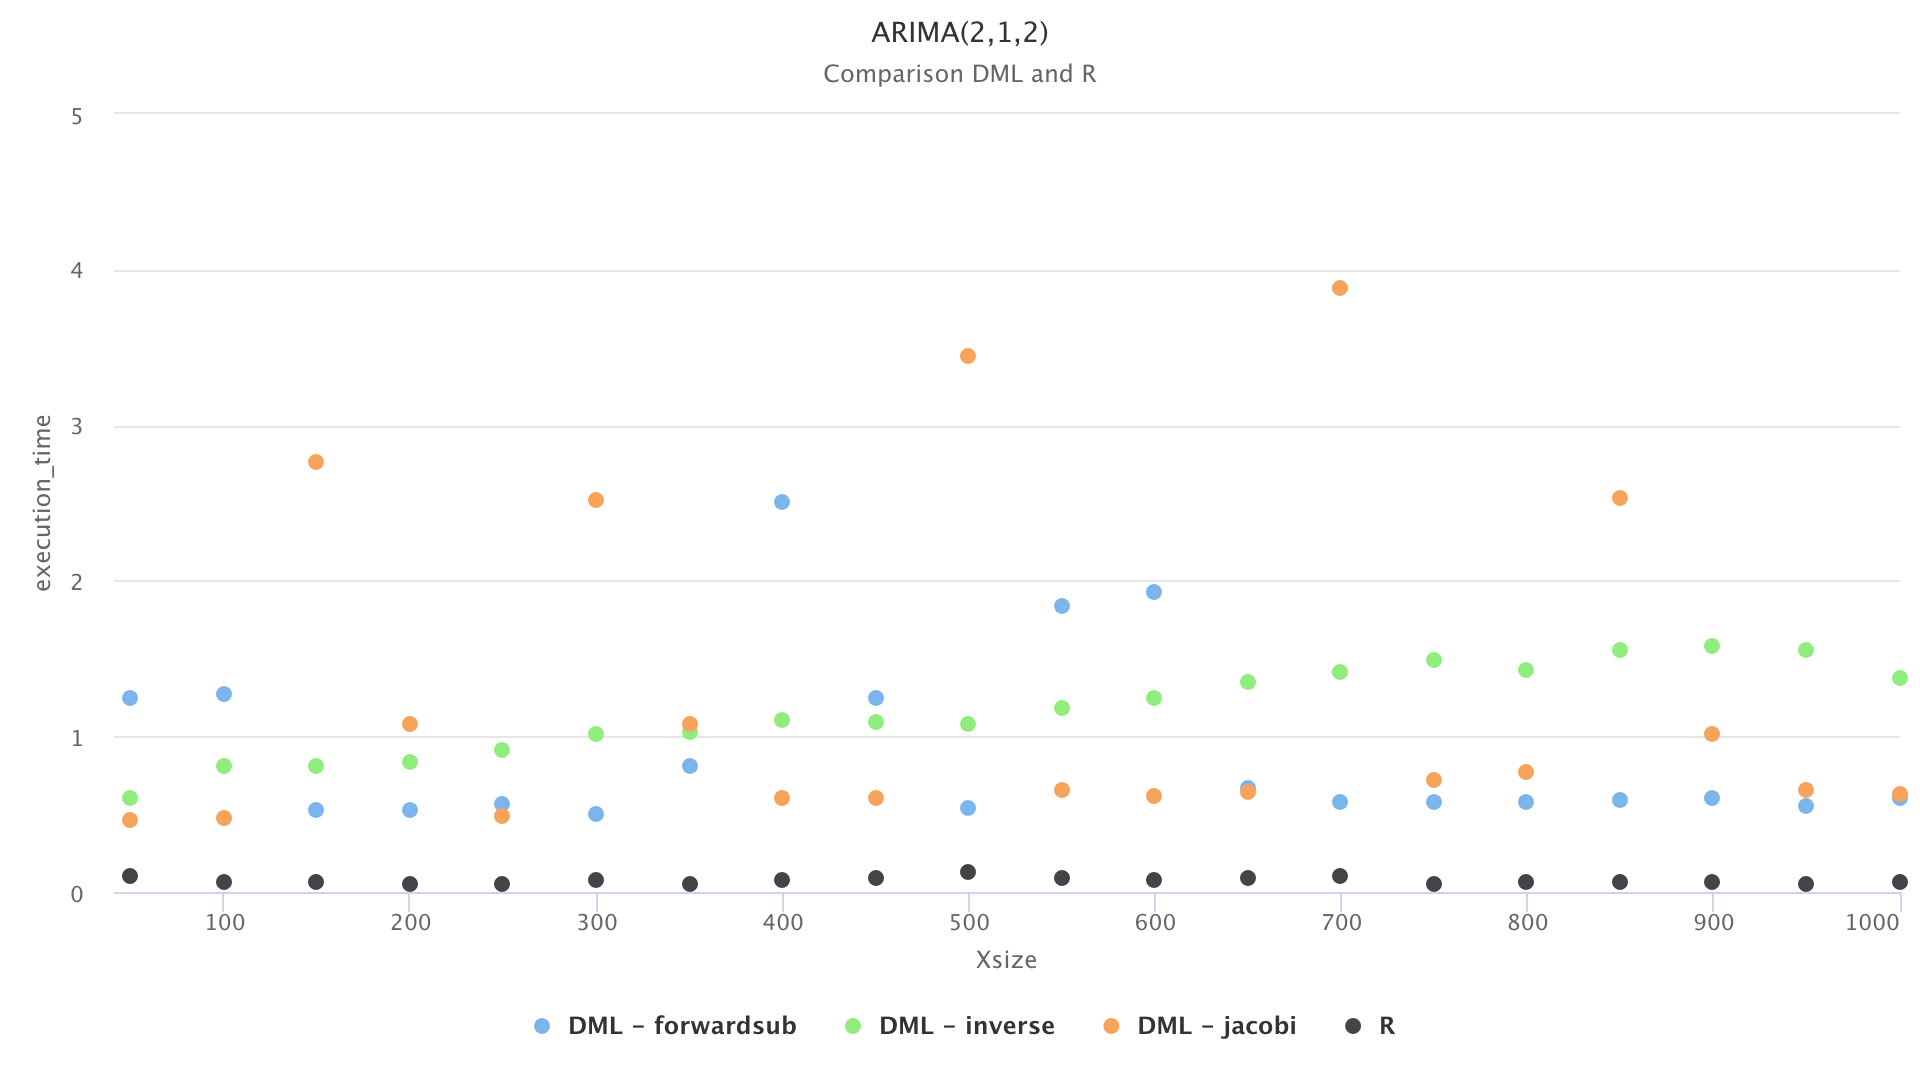
\includegraphics[width=\defaultsizeGraph]{images/arima212-exectime-scatter-all_small.png}}
	\caption{\textbf{Execution time} of ARIMA(2,1,2) for DML and R for time series with sizes \textbf{from $50$ to $1,000$} }
    \label{apx-fig:arima212-exectime-scatter-all_small}
\end{figure}

\begin{figure}[ht]
	\centering
	\scalebox{1}{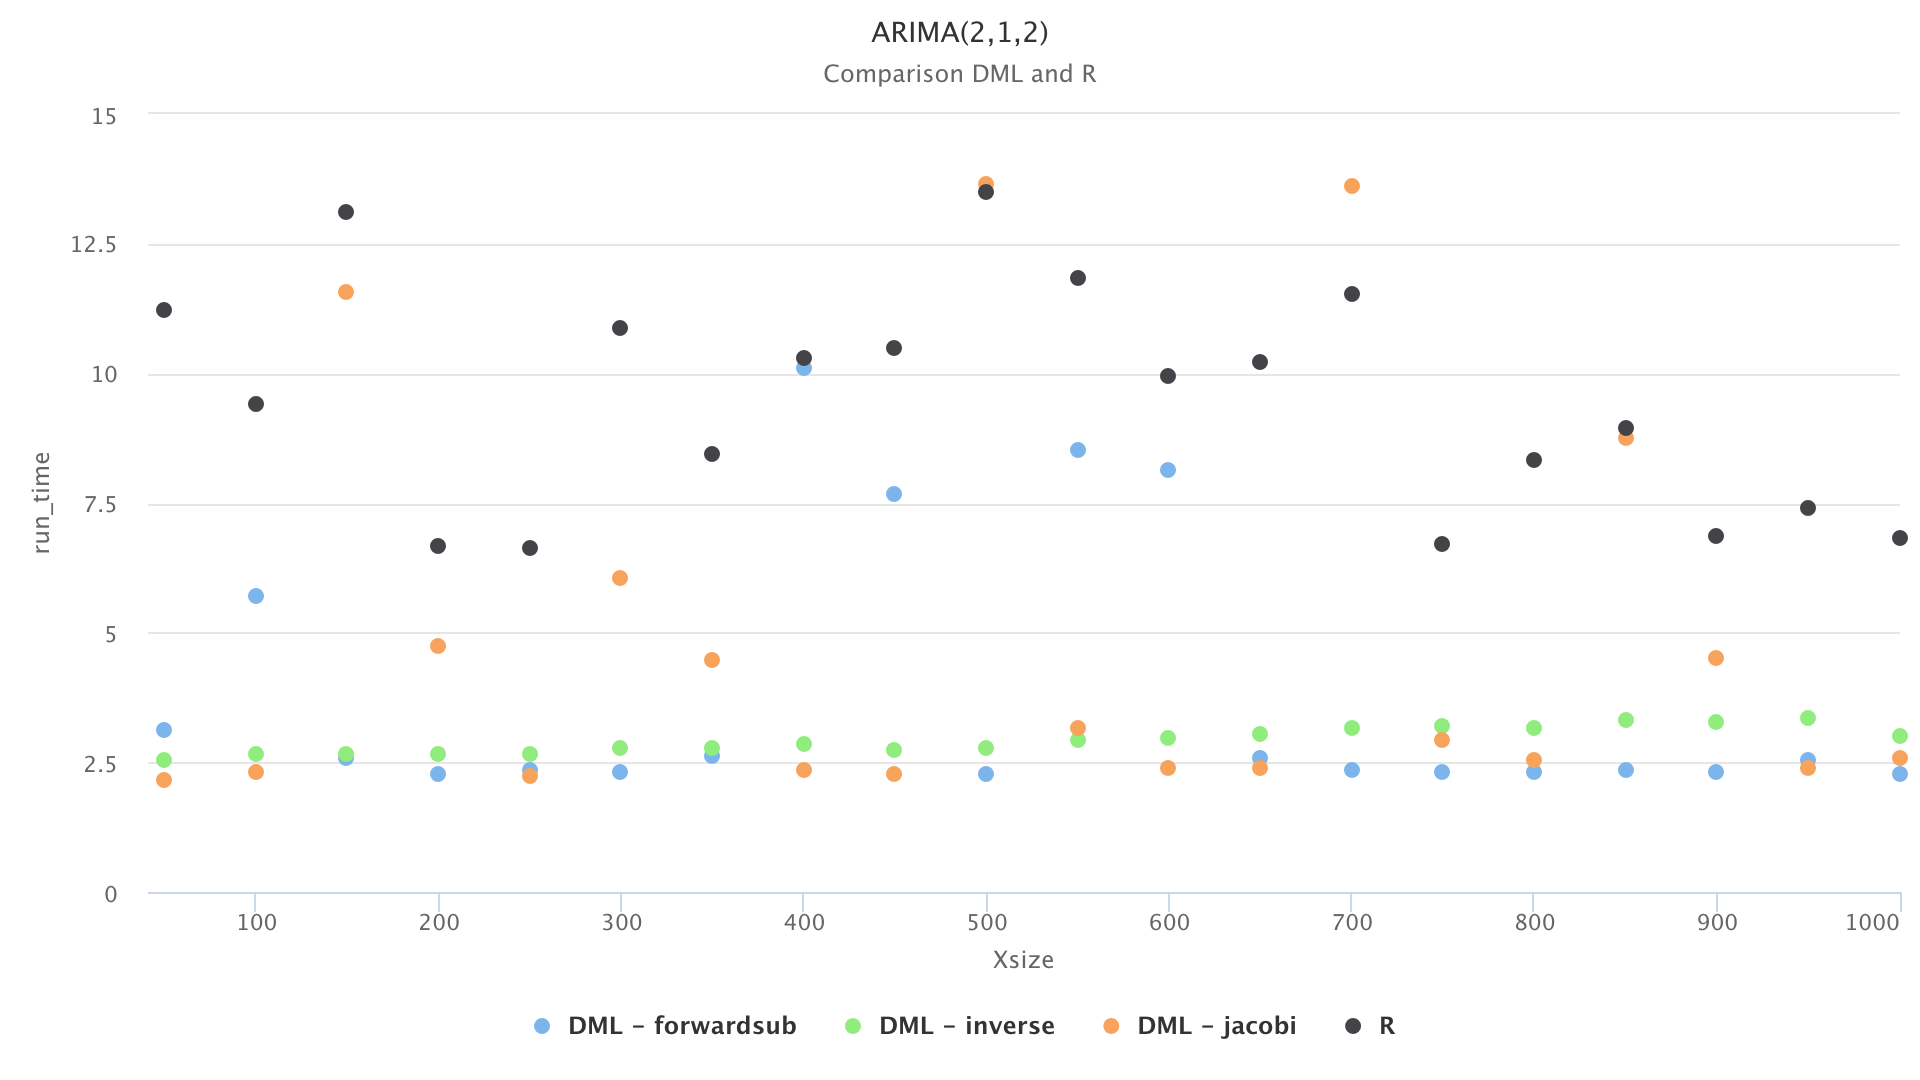
\includegraphics[width=\defaultsizeGraph]{images/arima212-runtime-scatter-all_small.png}}
	\caption{\textbf{Run time} of ARIMA(2,1,2) for DML and R for time series with sizes \textbf{from $50$ to $1,000$} }
    \label{apx-fig:arima212-runtime-scatter-all_small}
\end{figure}